\documentclass[conference]{IEEEtran}
\IEEEoverridecommandlockouts
\usepackage[strings]{underscore} % allow _ in ordinary text (incl. captions)


\usepackage[T1]{fontenc}
\usepackage[utf8]{inputenc} % for pdflatex

\usepackage{cite}
\usepackage{amsmath,amssymb,amsfonts}


\usepackage[hidelinks]{hyperref}
\usepackage{xurl}


\usepackage{booktabs}


\usepackage[ruled,vlined]{algorithm2e}
\newcommand{\code}[1]{\text{\footnotesize\texttt{\detokenize{#1}}}}
\newcommand{\codeline}[1]{\text{\ttfamily\footnotesize\detokenize{#1}}}

\newcommand{\regex}[1]{\lstinline[breaklines=true,basicstyle=\ttfamily\footnotesize,columns=fullflexible]{#1}}

\newcommand{\Set}[1]{$#1$}          % for sets/math inline
\newcommand{\bstr}[1]{\code{#1}}    % for byte/regex snippets

\SetAlFnt{\footnotesize}
\SetAlCapNameFnt{\footnotesize}
\SetAlCapFnt{\footnotesize}
\SetAlgoNlRelativeSize{-1}

\SetKw{KwAnd}{and}
\SetKw{KwOr}{or}
\SetKw{KwTo}{to}
\SetKw{KwIn}{in}
\SetKw{KwRet}{return}
\SetKwBlock{KwFn}{Function}{end}
\SetAlgoNlRelativeSize{-1}% slightly smaller line numbers in 2-col
\DontPrintSemicolon
% allow manual line breaks in algorithm function signatures
\newcommand{\argsbreak}{\\\hspace*{1.5em}}
% =======================================================

\usepackage{subcaption}
\usepackage{listings}
\lstset{
  basicstyle=\ttfamily\small,
  breaklines=true,
  frame=single,
  captionpos=b,
  aboveskip=0.8em,
  belowskip=0.8em,  
literate=%
    {Ö}{{\"O}}1
    {Ä}{{\"A}}1
    {Ü}{{\"U}}1
    {ß}{{\ss}}1
    {ü}{{\"u}}1
    {ä}{{\"a}}1
    {ö}{{\"o}}1
    {~}{{\textasciitilde}}1
}

\lstset{
    basicstyle=\ttfamily,
    breaklines=true,
    breakatwhitespace=true,
}

\usepackage{graphicx}
\usepackage{textcomp}
\usepackage{xcolor}
\def\BibTeX{{\rm B\kern-.05em{\sc i\kern-.025em b}\kern-.08em
    T\kern-.1667em\lower.7ex\hbox{E}\kern-.125emX}}
\begin{document}

\title{Excel Shrink: High-Performance Bytestream Parsing and Cleaning of Bloated Excel Spreadsheets}


\author{\IEEEauthorblockN{1\textsuperscript{st} Alexander Aue-Johr}
\IEEEauthorblockA{\textit{Institute of Rural Studies} \\
\textit{Thünen-Institute}\\
Braunschweig, Germany \\
0009-0001-8683-3630}

}

\maketitle

\begin{abstract}
  This paper introduces Excel Shrink, a tool designed to mitigate the pervasive problem of file bloat in Microsoft Excel spreadsheets. By analyzing Excel’s Office Open XML structure, we identify common sources of file bloat—such as cells, rows and columns that are empty, contain only whitespace, or have a style assigned that is invisible to the user. We propose a novel, streaming-based, regex-driven approach to reduce file size without altering the visual appearance. Our method employs a state-machine to manage the hierarchy of XML documents without relying on conventional XML parsing techniques by processing XML data incrementally at the bytestream level, and it leverages multithreading for performance improvements. This enables Excel Shrink to outperform Microsoft Excel when loading bloated files, and cleaning plus opening the shrunk file is faster than opening the bloated file directly. Evaluation on a dataset from the German Federal Statistical Office demonstrates that Excel Shrink can achieve file size reductions of up to 99.99\% and dramatically improve file loading times. This work not only provides practical insights for developers and end users but also opens new avenues for the efficient management of large-scale semi-structured data in spreadsheet environments.

\end{abstract}

\begin{IEEEkeywords}
component, formatting, style, styling, insert.
\end{IEEEkeywords}

  
\section{Introduction}

Spreadsheets such as Microsoft Excel are ubiquitous tools for ad-hoc data management and analysis across many domains—from finance to science—even among non-programmers  \cite{Bendre2015DataSpread}. It is estimated that over one-tenth of the world’s population uses spreadsheet software  \cite{Rahman2021NOAH}. However, the growing volumes of data have pushed these tools to their limits. Although modern Excel supports up to approximately one million rows per worksheet  \cite{Rahman2021NOAH, MicrosoftExcelSpecs}—a capacity unimaginable in earlier versions—simply increasing this limit does not ensure scalable performance. In practice, spreadsheets often become unresponsive when handling only a few hundred thousand rows  \cite{Bendre2015DataSpread,Budiu2019Hillview}, underscoring that while spreadsheets remain indispensable, they are inherently ill-suited for managing very large datasets compared to database systems. This tension between ease-of-use and scalability is the motivation for our research.

A particularly frustrating symptom of this limited scalability is \emph{Excel file bloat}—the tendency of \texttt{.xlsx} files to become excessively large and slow. Users frequently encounter workbooks that swell in size far out of proportion to any actual data contained within them \cite{someBloat}. Such bloat is not just a storage inconvenience; it also directly degrades performance, causing slow load/save times, heavy memory consumption, and delays in downstream data processing pipelines \cite{Mack2018Scalability}.
Understanding the causes of this bloat is therefore crucial. Prior reports and anecdotal evidence highlight several culprits. One common cause is excess formatting: Excel is notorious for retaining formatting in cells far beyond the used data range, silently inflating file size  \cite{Power2025WhyExcelFileLarge}. In effect, millions of “blank” cells may carry font, color, or border settings that contribute to the XML file, dramatically increasing the package size. Another cause is an overabundance of cell styles. Every unique combination of formatting (font, fill, border, etc.) is stored in a centralized style table; copying worksheets between workbooks or indiscriminate cell styling can accumulate tens of thousands of distinct styles. Excel allows up to ~64,000 unique cell styles, and hitting this limit or even a fraction of it can bloat the styles.xml part of the file and trigger errors.
\cite{Microsoft2024TooManyCellFormats}. In one documented case, Excel began warning the user that “this workbook has many duplicate styles which can slow performance,” prompting a cleanup of hundreds of extraneous style entries 
\cite{akira_hirai2024DuplicateStyles}. These examples underscore that Excel’s own features for flexibility (rich formatting, open XML storage) can turn into liabilities at scale.

The significance of the Excel bloat problem extends beyond file size annoyance—it poses broader scientific and technical challenges. First, it exemplifies the difficulties of managing large semi-structured data in a format not optimized for size or speed. The Office Open XML format (used by .xlsx) trades efficiency for interoperability, using verbose XML to represent spreadsheet content. When a workbook contains huge numbers of cells or lengthy text, the XML overhead (tags, attributes, and repetition) adds substantial bulk. A DOM parser, which builds an in-memory tree of the entire XML, can easily exhaust memory on multi-hundred-thousand-row sheets. For example, the memory consumption of a XML DOM parser (like \texttt{readxl}) can exceed ten times the size of the uncompressed worksheet (30 GB for 6.000.000 rows) \cite{Henze2022SheetReader}.
Streaming SAX parser avoids high memory usage but suffer from high CPU overhead due to handling a flood of callback events \cite{Henze2022SheetReader}. 

Such scenarios reflect the mismatch between Excel’s data model and big-data processing needs. Processing such bloated XML files is computationally expensive: parsing XML requires reading and interpreting deeply nested structures, which can strain I/O and memory. Indeed, standard XML parsing in memory (DOM) would load the entire spreadsheet into a tree, potentially consuming gigabytes of RAM for a bloated file. This is aggravated by Excel-specific XML components like the Shared Strings table (which holds all text entries) and the Styles table – both can grow very large and must be parsed or loaded before data can be accessed. As a result, reading a large .xlsx file with conventional libraries often becomes a bottleneck \cite{sancozta2020spout}. 
Second, the issue brings to light fundamental challenges in language theory and parsing. Excel’s file format—essentially a collection of XML documents—is a context-free language (Type-2 in the Chomsky hierarchy). Parsing such documents correctly requires managing recursive tag structures and dependencies (e.g., matching \texttt{<row>} and \texttt{</row>} tags or resolving references in shared string tables). It is mathematically impossible to accurately parse or validate XML using only regular expressions or simplistic line-by-line methods, since regular languages (Type-3) cannot handle arbitrary nested structures  \cite{Champion2021RegexTips,bobince2009RegexMatchOpenTags}. Consequently, robust tools for processing \texttt{.xlsx} files at scale must employ proper XML parsing strategies rather than relying on ad-hoc techniques.

This paper situates the Excel bloat problem within the context of database research and proposes technical approaches to mitigate it. We begin by analyzing the internal structure of Excel's Open XML format to identify the causes of file bloat and review related work and online resources regarding bloat in Excel files. We employ manual guides as well as tools such as Microsoft Excel’s Performance Tab and the Excel Inquire Add-In, and also trial versions of proprietary utilities like NXPowerLite Desktop, to assess their file size reduction capabilities.

After applying these manual guides and automatic tools to real-world Excel files, we perform a qualitative analysis of the XML code to examine the changes responsible for file size reduction. By comparing the visual integrity of the files before and after cleaning—and incrementally reverting modifications to pinpoint when visual errors disappeared—we gain insight into Excel's internal file structure and determine which cleanup operations are safe. Building on this reverse-engineering process, we identify a set of safe modifications and implement them in our own protptype tool - Excel Shrink Analyzer - using regular DOM-XML parsing for fast prototyping, to test these changes across a large number of files and validate the outcome by file size reduction and if the Spreadsheet still looks the same, to find the set of modifications that are safe and effective.

Following the prototype phase, we develop a tool applying the same modifications, but this time efficiently, using a state-machine-guided, regex-driven parser designed to clean bloated Excel files. This parser operates directly on the raw XML byte stream to overcome the limitations of conventional XML parsers when dealing with large, deeply nested structures. We evaluate the performance of this tool — referred to as Excel Shrink — on the same Dataset a series of Excel files by comparing the loading times of pre-cleaned files versus the original files when opened with standard libraries and Microsoft Excel itself.

To guide our study, we pose the following research questions:

\begin{enumerate}  
\item \textbf{(RQ1)} Are the root causes of Excel file bloat already well understood and documented in existing research, or is further empirical analysis needed to fully identify and quantify these causes?
\item \textbf{(RQ2)} Can a regex-driven, state-machine–guided parser overcome the typical limitations of regular expressions in processing structured XML data (e.g., prevent overmatching and preserve XML validity)?
\item \textbf{(RQ3)} Does precleaning bloated Excel files with such a method significantly improve overall loading time (\emph{i.e.}, cleaning + loading) compared to loading the original file directly in Excel?

\end{enumerate}

Through this exploration, we aim to bridge the gap between Excel’s convenience and the demands of very large-scale data management. Ultimately, our work aspires to improve the reliability and scalability of processing large Excel files by providing both developers and end users with actionable insights and practical tools. Developers gain a deeper understanding of the causes of file bloat and strategies for efficient cleanup, while Excel users receive a means to pre-clean files before further processing or to integrate Excel Shrink into automated workflows.




\section{Background}

\subsection{Excel's Open XML Format}

Excel workbooks (.xlsx) are stored in the Office Open XML format, which organizes spreadsheet data into multiple XML parts within a ZIP container. Notably, each worksheet is an XML file (sheet1.xml, sheet2.xml, etc.) containing the cell data (values, formulas) for that sheet  \cite{Microsoft2025SpreadsheetMLStructure}. In addition, there are global parts such as workbook.xml (overall workbook metadata like the names of the sheet and their order), styles.xml (definitions of cell, row and column formats), and sharedStrings.xml (the table of reoccuring texts in the file). The Shared String Table is especially important for understanding Excel’s storage mechanism. It is a construct that contains one instance of each unique text string appearing in the workbook. Instead of writing repeated text values in every cell, Excel stores each distinct string once in sharedStrings.xml and then references it by index from the sheet files. This design aims to reduce file size and memory usage when many cells contain duplicate text (e.g., a column of repeating categorical values)  \cite{Microsoft2025SharedStringTableClass, FasterCapital2024SharedStrings}. Each text cell in a sheet XML may look like <c r="A1" t="s"><v>42</v></c>. This means that the cell at position A1 does not contain the number 42 itself. Instead, the attribute t="s" marks the cell's content as a shared string reference — the <v> tag holds the index (here: 42) of the actual text stored in the file sharedStrings.xml. When Excel opens the worksheet, it looks up index 42 in that shared string table to retrieve and display the correct text in the cell. In scenarios with highly repetitive text, the shared string table yields smaller files.

Another central component is the Styles Part (styles.xml), which defines all cell formatting used in the workbook.
Excel supports rich formatting options for cells—such as fonts, colors, number formats, and borders—and manages these through style records. Each style record represents a specific combination of formatting properties and can be shared among multiple cells, rows, or columns.
Instead of duplicating formatting information, these elements simply reference the corresponding style record via the s attribute. \cite{Microsoft2025CellFormatClass}.

\subsection{Prior Observations and Literature}

Despite the prevalence of the Excel bloat problem in practice, there is scant academic literature that directly addresses it. To our knowledge, no peer-reviewed study thus far has focused on the internal inefficiencies of Excel's XML format or the mitigation of bloated spreadsheets. This is consistent with the fact that the database research community has traditionally viewed spreadsheets as end-user tools rather than enterprise-scale data management systems. However, indirectly, several lines of work and industry reports touch on related issues. Microsoft's official guidelines and support articles acknowledge problems such as the “Too many different cell formats” error (triggered by style overflow)
\cite{Microsoft2024TooManyCellFormats} and provide best practices for reducing workbook size (e.g., removing unused styles, turning off pivot cache, etc.). The Excel user community (blogs, forums) is rife with case studies of bloated files and remedies. For example, Power \cite{Power2025WhyExcelFileLarge}
 enumerates common reasons for oversized files and recommends using a ZIP tool to inspect which internal parts are largest - an approach that reveals whether data, formatting, or media are to blame. On Stack Overflow, Superuser and ExcelForum, numerous Q\&A threads document instances of mysterious file growth, often resolved by cleaning formats or rebuilding the workbook from scratch \cite{chrtak2024ExcelSheetBloated, SuperUser739577, SuperUser63119, ExcelForum1349596}
. These sources, while not formal research, provide valuable insight into the root causes of bloat and confirm that our problem formulation is grounded in reality. However the solutions they provide are often manual, some of them utalizing the Excel built in features, recently introduced features like the excel check performance tab or the older Excel Inquire Add In, which are not suitable for automation pipelines and not scalable for large numbers of files. Yet the causes in the XML structure of the Excel file is not addressed in these sources and can only be identified by reverse engeneering the cleanup tools or Microsoft excel itself by try and error removing parts of the XML file and checking if the file still looks the same.


In the academic sphere, there is growing recognition that spreadsheets and databases need not be disjoint worlds. Some research efforts have looked at enhancing spreadsheets to handle larger datasets by leveraging database technology in the background. DataSpread \cite{Bendre2015DataSpread} and Hillview \cite{Budiu2019Hillview} are two systems that retain an Excel-like interface but manage data in a relational database to improve scalability.

While these works are not about Excel's file format per se, they underscore a broader point: when spreadsheets approach the size of databases, one must apply database-like solutions. Our work aligns with this philosophy by treating Excel bloat and processing as a data management problem. Instead of dismissing bloated spreadsheets as user error, we view them as an important issue in large-scale semi-structured data processing that warrants efficient techniques.

 
\section{Related Work}
\label{sec:related-work}

A substantial body of research in top-tier venues (VLDB, SIGMOD, ICDE) has explored techniques to \emph{improve performance} on large or complex workbooks. There have also been several efforts to reduce \emph{Excel file size}, with various online resources discussing this topic. We briefly review key findings below, focusing on (i) methods for minimizing file size, (ii) approaches to accelerating computation and user interactions for large spreadsheets, (iii) optimizations for parsing the XML-based \texttt{.xlsx} format, and (iv) highlights of Aditya Parameswaran’s contributions in bridging spreadsheet and database technologies.

\textbf{Minimizing Excel File Size and Bloat.}
Microsoft’s transition from the binary \texttt{.xls} format to \texttt{.xlsx} (Office Open XML) introduced compression and a shared string table to reduce repeated data \cite{ecma2007openxml,Microsoft2007OpenXML}. Further reduction is achieved in the \texttt{.xlsb} (binary) format, which stores data in a compact binary container at the cost of certain compatibility constraints \cite{MicrosoftXLSB,Mack2018Scalability}.

However, there is a lack of peer-reviewed studies specifically quantifying how “bloat” (whitespace values, invisible formatting, rows and column definitions outside of the visible content) affects Excel file size \cite{lackOfStudies}. Instead, most advice on the subject comes from practitioners sharing their experiences. For example, Microsoft’s support article on cleaning excess cell formatting provides practical tips for reducing file size and improving performance \cite{MicrosoftXLSB}. Additionally, discussions on forums such as MrExcel illustrate that users have long noticed dramatic size reductions after clearing unused formatting or trimming the “used range” \cite{excelforum}. Popular Excel blogs from UpSlide \cite{upslide_blog}, The Bricks \cite{thebricks_blog} and Chandoo \cite{metadataBloat} further detail these methods based on accumulated user experience rather than formal experimentation.

Several proprietary tools have been developed to address Excel bloat automatically. Notable examples include UpSlide’s Automation Software, which offers a one-click “Smart Clean” feature \cite{upslide_blog}; NXPowerLite Desktop \cite{neuxpower2024nxpowerlite}; Sobolsoft’s Excel File Size Reduce Software \cite{sobolsoft}; and online services such as WeCompress \cite{wecompress}. Other tools, such as Kernel for Excel Repair \cite{kernel_excel}, have also been mentioned in user communities for their file compression capabilities.

Microsoft has also developed two tools to assist users. One such tool is \textbf{Excel Inquire}, an add-in introduced with Excel 2013 that provides a range of auditing features—including Workbook Analysis, Relationship Diagrams, and the Clean Excess Cell Formatting command. O'Beirne notes that the \textit{Clean Excess Cell Formatting} command removes excess formatting but does not indicate beforehand what will be cleared, nor does it report afterwards what was removed \cite{obeirne2013}.

More recently, Microsoft introduced the \textbf{Excel Performance Tab}, a built-in feature designed to monitor workbook performance by identifying inefficiencies and offering cleaning recommendations. However, the Performance Tab has received negative user feedback; several users report that its forced “Check Performance” pop-up and the associated reformatting remove intentional formatting and disrupt workflows \cite{mrexcel2024check,microsoft_cleanup} and also Excel users report that their pixel art is deleted \cite{mrexcel2024check} while the Microsoft Support Site even mentions a warning that pixel art will be removed by the tool \cite{microsoft_cleanup}.

In contrast, our paper provides a comprehensive scientific analysis of the root causes of Excel file bloat in XML-based workbooks. To address this gap, we introduce \textit{Excel Shrink}--- a command-line tool designed for automation pipelines. Unlike proprietary tools that are only accessible through a graphical user interface and sometimes remove too many elements (thereby altering the visual appearance) or too few (leaving the file size large), Excel Shrink selectively reduces file size by eliminating only those elements that do not affect the workbook’s visual integrity.

\textbf{Performance in Handling Large Spreadsheets.}
Rahman et al.~\cite{Rahman2020Benchmarking} conducted a comprehensive study comparing Excel, LibreOffice Calc, and Google Sheets on sizable datasets. They revealed that despite nominal row limits of one million, Excel’s GUI would often freeze with mere tens of thousands of rows or extended formula usage. Similar findings appear in other bench\-marking efforts 
\cite{Rahman2021NOAH}, 
highlighting the lack of indexing in typical spreadsheet software. Addressing this, “DataSpread”~\cite{Bendre2015DataSpread} (VLDB 2015) and “Hillview”~\cite{Budiu2019Hillview} (PVLDB 2019) offload data management to database engines or distributed clusters, respectively, while retaining a spreadsheet-like interface. These architectures stretch the notion of a “spreadsheet” to hundreds of millions (or billions) of rows by introducing parallelization, indexing structures, or incremental computation. In a different line of work, Bendre et al.~\cite{Bendre2019AntiFreeze} proposed an \emph{anti-freeze} model for formula recalculation, allowing asynchronous updates so the user interface does not lock while large spreadsheets recompute.

\textbf{Efficient Excel XML Processing.}
As modern Excel files (\texttt{.xlsx}) are essentially XML (SpreadsheetML) within a ZIP container, \emph{parsing} can become a bottleneck for large sheets. Classical DOM-based XML parsing can exhaust memory on multi-hundred-thousand-row spreadsheets, whereas SAX-based streaming, though more memory-friendly, suffers from high CPU overhead through numerous event callbacks 
\cite{Henze2022SheetReader}. 
A hybrid parser that combines DOM and SAX parsing, along with regular expressions for extracting the relevant file contents (e.g.\ \texttt{openxlsx} in R), can still be slow and memory-intensive under worst-case scenarios. By contrast, parsers relying exclusively on DOM parsing (e.g.\ \texttt{readxl} in R) may achieve faster runtime performance but often at the cost of higher memory usage. For instance, the memory consumption of \texttt{readxl} can exceed ten times the size of the uncompressed worksheet \cite{Henze2022SheetReader}. 
To address this, Henze et al.~\cite{Henze2022SheetReader} introduced \emph{SheetReader}, a specialized streaming parser that integrates decompression and XML scanning, and parallelizes chunk-level parsing. This yields dramatically lower memory footprints (often $40\times$ less) and faster loads ($3\times$ or more) compared to standard libraries.
Similar to this Excel Shrink also aims to reduce the memory footprint by streamwise processing of small chunks of the XML file and only keeping the relevant parts in memory.

\textbf{Comparisons of Parsing Approaches and Tools.}
These studies collectively show a trade-off between \emph{DOM-based} simplicity (at the cost of high memory usage) and fully \emph{SAX-based} pipelines (often incurring higher CPU overhead). Hybrid or domain-specific solutions—like regex-based extraction or streaming chunk processors that skip unneeded style markup—strike a middle ground 
\cite{openxlsx, Henze2022SheetReader}. 
Meanwhile, broad tool evaluations (Microsoft Excel vs.\ Google Sheets vs.\ LibreOffice Calc) confirm that no mainstream spreadsheet program handles large data sets efficiently out of the box 
\cite{Rahman2020Benchmarking}.

\textbf{Parameswaran’s Contributions: Bridging Spreadsheets and Databases.}
Aditya Parameswaran and collaborators have researched integrating spreadsheets with database backends to achieve both usability and scalability 
\cite{Bendre2015DataSpread, Bendre2018PDM}. 
\emph{DataSpread} preserves the familiar Excel-like interface while relying on a relational DBMS for storage and large-scale computations, enabling interactive performance even at billions of cells. This approach can be seen as bypassing Excel’s internal storage and recalculation limits by adopting database features (indexing, query optimization, concurrency control). In related work on “anti-freeze” recalculation, Parameswaran’s group explored asynchronous formula evaluation with incremental updates, preventing interface lock-ups for large or complex dependency graphs 
\cite{Bendre2019AntiFreeze}. 
Additionally, they highlight practical tactics like saving spreadsheets as binary (\texttt{.xlsb}) instead of \texttt{.xlsx} to mitigate bloat, limiting volatile formulas (e.g.\ \texttt{OFFSET}), and offloading heavy operations to databases where possible 
\cite{Mack2018Scalability}. 
All these strategies offer evidence that a combination of advanced parsing, background recalculation, and robust data management techniques can significantly enhance performance for real-world Excel workloads.

\textbf{Summary}
From straightforward file-format optimizations (\texttt{.xlsb} compression) to \emph{architectural} overhauls (DataSpread, Hillview) and specialized parsers (SheetReader), the research consensus is that Excel’s native engine and file format alone do not scale gracefully. Modern solutions increasingly combine streaming-based XML handling, database or distributed architectures, and asynchronous computation to push spreadsheet interactivity far beyond Excel’s historical limits. These insights strongly motivate the need for further improvements in \texttt{.xlsx} bloat reduction and high-performance parsing directly addressed by our proposed approach in this paper.

  

\section{Methodology}

\noindent Excel-Shrink is a stream-oriented XLSX cleaner that removes visually inconsequential XML
while preserving user-visible layout semantics
(e.g., fill/border styles that convey meaning),
and merges superfluous column definitions.
The system operates directly on the bytestream of the zipped OOXML container:
it parses \texttt{xl/workbook.xml}
and per-sheet \texttt{xl/worksheets/sheet*.xml} streams with regular expressions
instead of loading full XML trees into memory,
applies workbook-specific rewriting rules
derived from \texttt{xl/styles.xml} and \texttt{xl/sharedStrings.xml},
and re-emits a compacted archive.

We first formalise inputs and artefacts, then describe pipeline stages.

\subsection{Inputs, Outputs, and Notation}

\textbf{Inputs.}
\emph{Path} may be a single XLSX file, a directory, or an HTTPS/HTTP URL. Optional flags control recursion, multiprocessing, chunk size for streaming, sheet filters, and whether only the workbook is cleaned.

\textbf{Outputs.}
A cleaned XLSX written either to a file path or into an output directory, preserving all unmodified parts of the original OOXML.

\textbf{Core artefacts.}
\begin{itemize}
\item \emph{Workbook XML} (\texttt{xl/workbook.xml}): contains \texttt{<definedNames>} nodes.
\item \emph{Sheet XML} (\texttt{xl/worksheets/sheet*.xml}): contains \texttt{<cols>}, \texttt{<sheetData>}, \texttt{<mergeCells>}.
\item \emph{Styles} (\texttt{xl/styles.xml}): provides \texttt{<cellXfs>} with fill/border/apply flags.
\item \emph{Shared Strings} (\texttt{xl/sharedStrings.xml}): enables identification of pure-whitespace string table entries.
\end{itemize}

\noindent \textbf{Workbook-specific patterns.}
From \texttt{styles.xml} and \texttt{sharedStrings.xml} we derive:
\begin{enumerate}
\item sets of style indices with \emph{fill} or \emph{border} or with neither but \emph{font-only};
\item regex-like predicates for: (i) whitespace cells, (ii) consecutive empty cells/rows, (iii) attributes irrelevant for empty rows (\emph{spans}, vendor \emph{dyDescent}, etc.), and (iv) presence of \emph{hidden} rows/columns.
\end{enumerate}





\subsection{Deriving Workbook-Specific Patterns}
\label{sec:wb-patterns}


Our worksheet cleaning approach adopts a two-stage cleaning procedure based on a chunking strategy.
In the initial pre-processing phase, individual chunks are analysed
and cleaned using lightweight operations that do not require any global context
from the worksheet. Some of these operations require knowledge of the workbook structure,
others can be applied independently to each worksheet. Despite their simplicity,
these early operations are effective in eliminating a large portion of file bloat
from Excel spreadsheets.

Such operations involve the removal of visually inconsequential cells and rows—
cells that contain no content and no layout-relevant styling,
such as background fills or borders.
Font-only styling (e.g., font family or size) or filled  with
 whitespace characters  is insufficient to classify a cell as visually relevant.
By filtering out these cells during chunk-level processing,
we reduce both the computational burden and the memory footprint
of subsequent operations.

To identify and remove these visually inconsequential cells,
we need to know which styles correspond to visually empty formatting
and which shared strings correspond to whitespace-only content.

After extracting the style definitions from styles.xml
and the shared strings from sharedStrings.xml during the initial context extraction phase,
we can compile regex patterns that match cells and rows that are visually empty.
The  compilation of these patterns is summarised in Algorithm \ref{alg:build-wb-patterns}.

After extracting the style definitions from \texttt{styles.xml} and the shared strings
from \texttt{sharedStrings.xml} during the initial context extraction phase, we construct
several sets of indices that determine which cells or rows can safely be removed.
These sets and the resulting regular expressions are compiled in
Algorithm~\ref{alg:build-wb-patterns}.

Let \(S_{\mathrm{fb}}\) denote the set of all \emph{fill/border} style indices,
i.e.\ those \texttt{xf} records where either the \texttt{fillId} or
\texttt{borderId} attribute is non-zero.
For example, if the parsed style table (\texttt{styles.xml}) contains
\[
XFS[0].\mathrm{fillId}=0,
XFS[1].\mathrm{fillId}=3,
XFS[2].\mathrm{borderId}=2
\]
then \(S_{\mathrm{fb}}=\{1,2\}\).
These indices are joined into a single alternation string
\(\mathrm{FB} = \texttt{"1|2"}\),
which is used to form the regular expression
\[
p_{\text{fbh}} = \code{"(?:s="(?:1|2)"|"hidden="1")"}
\]
matching a row attribute that either has style with a set fill or border or a row attribute that is hidden used to find the last visually relevant row.

Analogously, \(S_{\mathrm{font}}\) represents the set of \emph{font-only} styles—
those that apply no fill or border at all.
For instance, if
\[
\begin{aligned}
XFS[3].\mathrm{fillId} &= 0, \quad XFS[3].\mathrm{borderId} = 0,\\
XFS[4].\mathrm{fillId} &= 0, \quad XFS[4].\mathrm{borderId} = 0,
\end{aligned}
\]

\noindent then \(S_{\mathrm{font}}=\{3,4\}\) is incorporated into the patterns

\[
\begin{aligned}
p_{\text{ra}} &= 
  \begin{aligned}[t]
  &\codeline{\s*(spans="[^"]+")}\\[-1pt]
  &\codeline{|[^:]+:dyDescent="[^"]*"}\\[-1pt]
  &\codeline{|s="(?:3|4)")}
  \end{aligned}
\\[4pt]
p_{\text{e}}  &= 
  \begin{aligned}[t]
  &\codeline{(?:<c\b(?:(?![^>]*s=)[^>]*)}\\[-1pt]
  &\codeline{|[^>]*s="(?:3|4)"}\\[-1pt]
  &\codeline{[^>]*)/>)+}
  \end{aligned}
\end{aligned}
\]

\noindent which respectively match redundant row attributes and
consecutive font-only empty cells.






Next, \(W\) is the set of \emph{shared string indices} that correspond to
whitespace-only values (e.g.\ cells containing a single space or tab).
For example, if \texttt{sharedStrings.xml} contains
\begin{lstlisting}[language=XML,basicstyle=\ttfamily\scriptsize,frame=none]
<si><t> </t></si>
<si><t>  </t></si>
<si><t>hello</t></si>
\end{lstlisting}
then \(W=\{0,1\}\) and
\(\mathrm{WS}=\texttt{"0|1"}\).

These indices produce the regexes
\[
\begin{aligned}
p_{\text{ws}} &= \codeline{<v>(?:0|1)</v>}\\
p_{\text{wc}} &= \codeline{(<c\b[^>]*t="s"[^>]*?)><v>(?:0|1)</v></c>}
\end{aligned}
\]
which match the corresponding whitespace value tags and their enclosing
\texttt{<c>} elements.

All resulting expressions \(p_{\text{ra}}\), \(p_{\text{e}}\),
\(p_{\text{fbh}}\), \(p_{\text{ws}}\), and \(p_{\text{wc}}\)
are compiled into the regex set \(R\).
Together with the mapping $XFS$ from style IDs to \texttt{xf} records,
they form a complete \emph{pattern context} that drives the subsequent
byte-stream cleaning phase.
This allows the cleaner to efficiently detect and remove visually empty cells
and rows purely through regular-expression matching—without ever parsing
the XML structure.



\begin{algorithm}
\DontPrintSemicolon
\SetKwFunction{ParseCellXfs}{parseCellXfs}
\SetKwFunction{IdxWhitespaceSI}{indicesOfWhitespaceSI}
\SetKwFunction{Join}{join} % textual join with "|"
\SetKwProg{Fn}{Function}{:}{}

\Fn{\textsc{BuildWorkbookPatterns}($B_{\text{stylesXml}}, B_{\text{sharedStringsXml}}$)}{

  % parse cellXfs
  $xfs \gets \operatorname{parseCellXfs}(B_{\text{stylesXml}})$\;

  % index sets
  $S_{\mathrm{fb}} \gets \{\, i \mid xfs[i].\mathrm{fillId}\neq 0 \lor xfs[i].\mathrm{borderId}\neq 0 \,\}$\;
  $S_{\mathrm{font}} \gets \{\, i \mid (xfs[i].\mathrm{fillId}\in\{0,\mathtt{None}\}) \land (xfs[i].\mathrm{borderId}\in\{0,\mathtt{None}\}) \land \neg xfs[i].\mathrm{applyFill} \land \neg xfs[i].\mathrm{applyBorder} \,\}$\;

  % shared strings indices that are whitespace-only
  $W \gets \textsc{IndicesOfWhitespaceSI}(B_{\text{sharedStringsXml}})$\;

  % optional: finite map view of xfs (for exposition)
  $\mathsf{XFS} \gets \{\, "0"\mapsto xfs[0],\ "1"\mapsto xfs[1],\ldots \,\}$\;

  %%% OFS + (rho1, rho2)
  \uIf{$|S_{\mathrm{font}}|>0$}{
    $\mathrm{OFS} \gets \Join(S_{\mathrm{font}}, \texttt{|})$\;
    $p_{\text{ra}} \gets$ \code{'\s*(\bspans="[^"]+?"|' + }\\
    \code{   '\b[^\s:]*?:dyDescent="[^"]*"|' + } \\
    \code{   '\bs="(?:' + OFS + ')")'}\;
    $p_{\text{e}} \gets$ \code{'(?:<c\b(?:(?![^>]*\bs=)[^>]*|[^>]*' + } \\
    \code{ '\bs="(?:' + OFS + ')"[^>]*)/>)+'}\;
  }\Else{
    $p_{\text{ra}} \gets$ \code{'\s*(\bspans="[^"]+?"|' + } \\
    \code{      '\b[^\s:]*?:dyDescent="[^"]*")'}\;
    $p_{\text{e}} \gets$ \code{'(?:<c\b(?![^>]*\bs=)[^>]*/>)+'}\;
  }

  %%% FB + (rho3)
  \uIf{$|S_{\mathrm{fb}}|>0$}{
    $\mathrm{FB} \gets \Join(S_{\mathrm{fb}}, \texttt{|})$\;
    $p_{\text{fbh}} \gets$ \code{'(?:s="(?:' + FB + ')"|"hidden="1")'}\;
  }\Else{
    $p_{\text{fbh}} \gets$ \code{'"hidden="1"'}\;
  }

  %%% WS + (rho4, rho5)
  \uIf{$|W|>0$}{
      $\mathrm{WS} \gets \Join(W, \texttt{|})$\;
    $p_{\text{ws}} \gets$ \code{'<v>(?:' + WS + ')</v>'}\;
    $p_{\text{wc}} \gets$ \code{'(<c\b[^>]*?\bt="s"[^>]*?)><v>(?:'} \\
    \code{   + WS + ')</v></c>'}\;
  }\Else{
    $p_{\text{ws}} \gets \text{None}$\;
    $p_{\text{wc}} \gets \text{None}$\;
  }

  $\mathcal{P} \leftarrow \{p_{\text{ra}},p_{\text{e}},p_{\text{fbh}},p_{\text{ws}},p_{\text{wc}}\}$ with \textsc{compile} for all non-\texttt{None}\;

  \KwRet $\langle \mathcal{P},\ $XFS$\rangle$\;

}
\caption{Consolidated construction: compute alternations and build dependent regexes in the same branch.}
\label{alg:build-wb-patterns}
\end{algorithm}



These patterns parameterise all sheet and workbook transformations that follow, ensuring we preserve semantically relevant visual styling.


\newcommand{\xtag}[1]{\text{\scriptsize\texttt{#1}}} % for literal XML tags
\newcommand{\concat}{\mathbin{\|}}                   % byte-sequence 

\begin{algorithm}
  \caption{Streaming extraction of sheet components}
  \label{alg:preprocess}
  \DontPrintSemicolon
  \SetKwProg{Fn}{Function}{:}{}
  \SetKwFunction{NextTag}{$\mathrm{nextTag}$}
  \SetKwFunction{Consume}{$\mathrm{consumeUntil}$}
  \SetKwFunction{ParseCols}{$\mathrm{parseColDefs}$}
  \SetKwFunction{PreSD}{$\mathrm{preProcessSD}$}
  \SetKwFunction{TrackMC}{$\mathrm{trackMaxMerge}$}
\SetKwFunction{ConsumeSD}{ConsumeSheetData}
\SetKwFunction{ConsumeCols}{ConsumeCols}
\SetKwFunction{ConsumeMC}{ConsumeMergeCells}

  %%%%%%%%%%%%%%%%%%%%%%%%%%%%%%%%%%%%%%%%%%%%%%%%%%%%%%%%%%%%%%%%%%%%%%%%%%%%%%
  % Main procedure
  %%%%%%%%%%%%%%%%%%%%%%%%%%%%%%%%%%%%%%%%%%%%%%%%%%%%%%%%%%%%%%%%%%%%%%%%%%%%%%
  \Fn{\textsc{PreprocessSheetStreamwise}($\mathit{sheetStream}, \mathcal{P}, \mathsf{chunkSize}$)}{

    % buffers / accumulators
    $state \gets \mathsf{IN\_WORKSHEET}$;\quad $b \gets \epsilon$;\;
    $B_{\text{preCols}},\ B_{\text{cols}},\ B_{\text{preSD}},\ B_{\text{sheetData}},\ B_{\text{preMC}},\ B_{\text{mergeCells}},\ B_{\text{tail}} \gets \epsilon$;\;

    % tracking structures
    $\mathcal{T} \gets \varnothing$;\quad \emph{processed tags} \;
    $\mathcal{T} \gets \varnothing$;\quad \emph{processed tags} \;

    $\mathcal{D}_col \gets \mathrm{newRangeMap}()$;\quad \emph{column defs (map)} \;
    $m_{\max}\gets \bot$;\;

    % literals / observers
    $\mathcal{O} \gets \{\xtag{<cols>},\ \xtag{<sheetData>},\ \xtag{<mergeCells>},\ \xtag{</worksheet>}\}$;\;

    \While{$state \neq \mathsf{FOUND\_END}$}{
      $b \gets b \concat \mathrm{read}(\mathit{sheetStream}, \mathsf{chunkSize})$;\;

      \uIf{$state = \mathsf{IN\_WORKSHEET}$}{
        $R \gets \mathcal{O} \smallsetminus \mathcal{T}$;\;
        $\langle tag,\ i_{\text{tag}},\ j_{\text{tag}} \rangle \gets \NextTag(b, R)$;\;

        \uIf{$tag \neq \bot$}{
          \lIf{$tag = \xtag{<cols>}$}{
            $B_{\text{preCols}} \gets B_{\text{preCols}} \concat b[0{:}i_{\text{tag}})$
          }
          \lIf{$tag = \xtag{<sheetData>}$}{
            $B_{\text{preSD}} \gets B_{\text{preSD}} \concat b[0{:}i_{\text{tag}})$
          }
          \lIf{$tag = \xtag{<mergeCells>}$}{
            $B_{\text{preMC}} \gets B_{\text{preMC}} \concat b[0{:}i_{\text{tag}})$
          }

          % drop the consumed prefix incl. the tag
          $b \gets b[j_{\text{tag}}{:}|b|)$;\;

          % state transition + bookkeeping
          $state \gets \mathrm{nextState}(tag)$;\;
          $\mathcal{T} \gets \mathcal{T} \cup \{tag\}$;\;
        }
      }

      \uElseIf{$state = \mathsf{IN\_COLS}$}{
        $\langle c,\ b,\ state,\ \mathcal{D}_col \rangle \gets \textsc{ConsumeCols}(b,\ \mathcal{P}, \mathcal{D}_col)$\;
        $B_{\text{cols}} \gets B_{\text{cols}} \concat c$\;
      }

\uElseIf{$state=\mathsf{IN\_SHEETDATA}$}{
  $\langle c,\ b,\ state\rangle \gets \textsc{ConsumeSheetData}(b,\mathcal{P})$\;
  $B_{\text{sheetData}} \gets B_{\text{sheetData}} \concat c$\;
}

      \uElseIf{$state = \mathsf{IN\_MERGECELLS}$}{
        $\langle c,\ b,\ state,\ m_{\max} \rangle \gets \textsc{ConsumeMergeCells}(b,\ m_{\max})$\;
        $B_{\text{mergeCells}} \gets B_{\text{mergeCells}} \concat c$\;
      }

      \Else{
        % no further structural tag: everything remaining is tail
        $B_{\text{tail}} \gets B_{\text{tail}} \concat b[0{:}|b|)$;\;
        $b \gets \epsilon$;\;
        \textbf{break}\;
      }
    }

  $\mathcal{M} \leftarrow \{\mathcal{D}_col,m_{\max}\}$\;


\Return $\textsf{Preprocessed}\left(
  \vcenter{\hbox{$
    \begin{alignedat}{1}
      &B_{\mathrm{preCols}},\ B_{\mathrm{cols}},\ B_{\mathrm{preSD}},\ B_{\mathrm{sheetData}},\\
      &B_{\mathrm{preMC}},\ B_{\mathrm{mergeCells}},\ B_{\mathrm{tail}},\mathcal{M}
    \end{alignedat}
  $}}
\right)$;\;

  }

  \BlankLine

\Fn{\textsc{ConsumeSheetData}($b,\mathcal{P}$)}{
  $i \gets \operatorname{find}\!\bigl(b,\xtag{</sheetData>}\bigr)$\;
  \lIf{$i \ge 0$}{
    \KwRet $\langle \textsc{PreProcessSD}(b[0{:}i],\mathcal{P}),\ b[i{:}],\ \mathsf{IN\_WORKSHEET}\rangle$
  }
  $k \gets \operatorname{rfind}\!\bigl(b,\xtag{<row}\bigr)$\;
  \lIf{$k \ge 0$}{
    \KwRet $\langle \textsc{PreProcessSD}(b[0{:}k],\mathcal{P}),\ b[k{:}],\ \mathsf{IN\_SHEETDATA}\rangle$
  }
  \KwRet $\langle \epsilon,\ b,\ \mathsf{IN\_SHEETDATA}\rangle$\;
}

  %%%%%%%%%%%%%%%%%%%%%%%%%%%%%%%%%%%%%%%%%%%%%%%%%%%%%%%%%%%%%%%%%%%%%%%%%%%%%%
  % Column-definition parser (map builder)
  %%%%%%%%%%%%%%%%%%%%%%%%%%%%%%%%%%%%%%%%%%%%%%%%%%%%%%%%%%%%%%%%%%%%%%%%%%%%%%
  %\Fn{\ParseCols{$x, \mathcal{P}$}}{
  %  $\mathcal{E} \gets \mathrm{newRangeMap}()$;\;
  %  \ForEach{$c \gets \mathrm{nextCol}(x)$}{
  %    $(\texttt{min},\texttt{max},\texttt{style},\texttt{hidden}) \gets \mathrm{fields}(c)$\;
  %    $xf \gets \mathrm{xfLookup}(\texttt{style},\ \mathcal{P})$\;
  %    $\mathrm{addRange}(\mathcal{E},\ \texttt{min},\ \texttt{max},\ xf,\ \texttt{hidden})$\;
  %  }
  %  $\mathrm{finalise}(\mathcal{E})$;\;
  %  \KwRet $\mathcal{E}$\;
  %}

\end{algorithm}


\subsection{Streaming Sheet Pre-processing}



We implement our spreadsheet parser streaming-based, processing the XML data incrementally to minimize memory consumption and permit early discarding of unnecessary file sections. Below, we focus on how the parser transitions between states (i.e., how each state function decides to proceed), deferring lower-level details of in-state processing until later sections (Algorithm \ref{alg:preprocess}).

\paragraph{States Overview}
We define six main states in our parser:
\begin{itemize}
  \item \texttt{BEFORE\_COLS}: The parser has not yet encountered the \texttt{<cols>} element. It searches for either \texttt{<cols>} or \texttt{<sheetData>}.
  \item \texttt{IN\_COLS}: The parser found \texttt{<cols>} and is processing column definitions.
  \item \texttt{BEFORE\_SHEET\_DATA}: The parser has finished reading (or did not detect) the \texttt{<cols>} node and is searching for the first \texttt{<sheetData>} element.
  \item \texttt{IN\_SHEET\_DATA}: The parser is processing the main worksheet data (rows and cells).
  \item \texttt{AFTER\_SHEET\_DATA}: The parser has detected the closing \texttt{</sheetData>} and is collecting any subsequent chunks until the end of the file.
  \item \texttt{END\_OF\_FILE}: The parser has reached the end of the stream, and no further parsing is needed.
\end{itemize}

\paragraph{In between nodes}
In \texttt{BEFORE\_COLS}, \texttt{BEFORE\_SHEET\_DATA}, or \texttt{AFTER\_SHEET\_DATA}, the parser looks for tag boundaries (e.g., \verb|<cols>|, \verb|<sheetData>|) or the end of file. When it detects such a tag at position \verb|i| in the buffer:
\begin{enumerate}
  \item It \emph{cuts} the buffer at \verb|i|, splitting the buffer into two segments:
   (1) from the start to the end of the located tag, and (2) the bytes after that tag.
  \item It returns the first segment as a chunk to add to the output, which the parser outputs or processes for the current state.
  \item The second segment becomes the updated buffer, ensuring the XML node boundary is never split across segments.
\end{enumerate}
If the parser fails to find any relevant tag or end of file, it returns no new output chunk, remains in the same state and leaves the buffer unmodified. This ensures that subsequent incoming data can be appended, eventually providing enough content to match the target boundary.

\paragraph{In column definition node}
In \texttt{IN\_COLS}, the parser searches for \verb|</cols>| or any \verb|<col .../>| elements. On detecting \verb|</cols>|, it cuts the buffer right before the closing tag and transitions to \texttt{BEFORE\_SHEET\_DATA}. If it does not find the closing tag but locates complete \verb|<col .../>| elements, those are consumed and removed from the buffer as a clean cut. If no match is found, the buffer remains unchanged, waiting for more data to complete the matching.


\begin{algorithm}
\caption{PreProcessSD — streaming prefilters for \texttt{<sheetData>} chunks}
\label{alg:presd}
\DontPrintSemicolon
\SetKwFunction{PreSD}{preProcessSheetData}
\SetKwFunction{Compile}{compile}
\SetKwProg{Fn}{Function}{:}{}


\KwData{  
  $p_{\text{hid}} \gets$ compile( \;
    \code{'(<row\b[^/>]*?\bhidden="1"[^/>]++' + }  \\
    \code{'(?:/>|>(?:(?!(?:</row>|<v>)).)++</row>))' + }  \\
    \code{'(?:<row\b[^/>]*?\bhidden="1"[^/>]++' +}  \\
    \code{'(?:/>|>(?:(?!(?:</row>|<v>)).)++</row>))+'}) \;
  }%
  
  \BlankLine

  
\Fn{\textsc{PreProcessSD}($b$, $\mathcal{P}$)}{
  %\tcp{Input: $x$ = \texttt{<sheetData>} bytes (row-aligned).}
  %\tcp{Params: $\mathcal{P}$ = pattern pack with fields
  %$\{p_{\text{ws}}, p_{\text{wc}}, p_{\text{e}}\}$: whitespace, whitespace-cell, consecutive-font-only-styled-empty-cells.}

  

  %\tcp{Local constant: collapse consecutive hidden rows (keep \textbackslash1).}

  

  \BlankLine
  %\tcp{Coalesce consecutive hidden rows.}
  \If{$\operatorname{has}(b,\ \xtag{hidden="1"})$}{
    $b \gets \operatorname{sub}(p_{\text{hid}}, "\textbackslash1", b)$\;
  }

  \BlankLine
  %\tcp{Replace whitespace shared-string cells.}
  \If{$\operatorname{has}(\mathcal{P}.p_{\text{ws}})\ \land\ \operatorname{has}(\mathcal{P}.p_{\text{wc}})$}{
    \If{$\operatorname{match}(\mathcal{P}.p_{\text{ws}}, b)$}{
      $b \gets \operatorname{sub}(\mathcal{P}.p_{\text{wc}}, "\textbackslash1/>", b)$\;
    }
  }

  \BlankLine
  %\tcp{Drop consecutive empty, layout-neutral cells.}
  \If{$\operatorname{has}(b,\ \xtag{<c})$}{
    $b \gets \operatorname{sub}(\mathcal{P}.p_{\text{e}}, "", b)$\;
  }

  \BlankLine
  %\tcp{Return cleaned chunk.}
  \KwRet $b$\;
}
\end{algorithm}



\paragraph{In sheet data node}
While \texttt{IN\_SHEET\_DATA}, the parser similarly looks for \verb|</sheetData>| or row boundaries \texttt{<row ...>...</row>} (or \texttt{<row .../>}). If \verb|</sheetData>| is found, the parser cuts the buffer at that tag and transitions to \texttt{AFTER\_SHEET\_DATA}. If no boundary is present yet, the buffer remains unaltered to combine with future data chunks.

\paragraph{Ensuring ``Clean Cuts'' within the Streaming Buffer}
Our parser reads raw XML data into a working buffer and ensures each XML node boundary is cleanly preserved, so no node is split across buffers. Each state-transition function adheres to this principle, only cutting when a relevant XML tag is fully identified. 

\paragraph{Buffer Updates and State Progress}
By constraining parsing decisions to these well-defined cuts, the parser never splits an XML node across multiple buffers. Each function (1) cuts on the matching tag boundary and updates the parser state, or (2) leaves the buffer intact if no complete boundary is found, thus allowing the next chunk to complete it. This way the parser can process the XML incrementally without needing to store the entire document in memory and it is ensured that the regular expressions dont't fail due to incomplete XML nodes and also only the regular expressions that are relevant to the current section of the document are applied, incresing the performance in comparison to applying all regular expressions on the whole document.


\begin{algorithm}[t]
\caption{SplitSheetDataRanges — compute \emph{cellsRange} and trailing \emph{rowsRange}}
\label{alg:split-sheetdata}
\DontPrintSemicolon
\SetKwProg{Fn}{Function}{:}{}
\SetKw{Raise}{\textbf{raise}}

\Fn{\textsc{SplitSheetDataRanges}($B_{\mathrm{sheetData}}$, $\mathcal{P}$)}{
  %\tcp{Input $sheet_data_bytes$: bytes of the \xtag{<sheetData>} node.}
  %\tcp{$patterns.p_{\mathrm{fbh}}$: compiled regex for \code{s="FB"} or \code{hidden="1"}.}

  \BlankLine
  %\tcp{1) Find the end of the last row that still contains a cell.}
  $i_{\mathrm{lastC}} \gets \operatorname{rfind}(B_{\mathrm{sheetData}},\ \code{"<c "})$\;
  \If{$i_{\mathrm{lastC}} = -1$}{
    $i_{\mathrm{cellsEnd}} \gets -1$\;
  }
  \Else{
    $j \gets \operatorname{find}(B_{\mathrm{sheetData}},\ \code{"</row>"},\ i_{\mathrm{lastC}})$\;
    \If{$j=-1$}{
          \Raise{Error: "no </row> after last <c"}{}
      }
    $i_{\mathrm{cellsEnd}} \gets j + |\code{"</row>"}|$\;
  }

  \BlankLine
  %\tcp{2) Scan for last visible attribute (fill/border style or \code{hidden="1"}).}
  $i_{\mathrm{visAttr}} \gets i_{\mathrm{cellsEnd}}$\;
  $m_{\mathrm{last}} \gets \bot$\;
  \ForEach{$m \in \operatorname{finditer}(patterns.p_{\mathrm{fbh}},\ B_{\mathrm{sheetData}},\ \text{start}=i_{\mathrm{cellsEnd}})$}{
    $m_{\mathrm{last}} \gets m$\;
  }
  \If{$m_{\mathrm{last}} \neq \bot$}{
    $i_{\mathrm{visAttr}} \gets \max(i_{\mathrm{visAttr}},\ \textsf{start}(m_{\mathrm{last}}))$\;
  }

  \BlankLine
  %\tcp{3) From that anchor, find the end position of the last visible row.}
  $j_{\mathrm{close}} \gets \operatorname{find}(B_{\mathrm{sheetData}},\ \code{"</row>"},\ i_{\mathrm{visAttr}})$\;
  $j_{\mathrm{self}}  \gets \operatorname{find}(B_{\mathrm{sheetData}},\ \code{"/>"},\ i_{\mathrm{visAttr}})$\;

  \uIf{$j_{\mathrm{close}} \neq -1 \land j_{\mathrm{self}} \neq -1$}{
    \uIf{$j_{\mathrm{close}} < j_{\mathrm{self}}$}{
      $i_{\mathrm{rowsEnd}} \gets j_{\mathrm{close}} + |\code{"</row>"}|$\;
    }\Else{
      $i_{\mathrm{rowsEnd}} \gets j_{\mathrm{self}} + |\code{"/>"}|$\;
    }
  }
  \uElseIf{$j_{\mathrm{close}} = -1 \land j_{\mathrm{self}} \neq -1$}{
    $i_{\mathrm{rowsEnd}} \gets j_{\mathrm{self}} + |\code{"/>"}|$\;
  }
  \uElseIf{$j_{\mathrm{close}} \neq -1 \land j_{\mathrm{self}} = -1$}{
    $i_{\mathrm{rowsEnd}} \gets j_{\mathrm{close}} + |\code{"</row>"}|$\;
  }
  \Else{
    \Raise{Error: "no </row> or /> after last anchor"}{}
  }

  \BlankLine
  %\tcp{4) Slice out the two ranges.}
  \uIf{$i_{\mathrm{cellsEnd}} = -1$}{
    $\textit{cellsRange} \gets \epsilon$\;
  }\Else{
    $\textit{cellsRange} \gets B_{\mathrm{sheetData}}[0 : i_{\mathrm{cellsEnd}}]$\;
  }

  $i_{\mathrm{rowsStart}} \gets \max(0,\ i_{\mathrm{cellsEnd}})$\;
  \uIf{$i_{\mathrm{rowsEnd}} = -1$}{
    $\textit{rowsRange} \gets \epsilon$\;
  }\Else{
    $\textit{rowsRange} \gets B_{\mathrm{sheetData}}[i_{\mathrm{rowsStart}} : i_{\mathrm{rowsEnd}}]$\;
  }

  \BlankLine
    \KwRet $\langle \textit{cellsRange},\ \textit{rowsRange}\rangle$\;

}
\end{algorithm}



The sub-routine \textsf{preProcessSheetData} (Algorithm \ref{alg:presd}) performs three linear passes over chunks:
(i) collapse explicit whitespace cells discovered via shared-strings indices,
(ii) remove consecutive empty cells (either styleless or font-only),
and (iii) opportunistically remove runs of hidden rows
while retaining the first sentinel
when needed to preserve row height/visibility semantics.

Two of these transformations depend on workbook-specific patterns
derived from \texttt{styles.xml} and \texttt{sharedStrings.xml} as described in Section
\ref{sec:wb-patterns}. Those are the removal of explicit whitespace cells
and the removal of consecutive empty cells with font-only or no styling.
Before these, we can also collapse consecutive hidden rows
into a single sentinel row.
In Excel’s internal representation,
rows can be marked as hidden using the attribute \xtag{hidden="1"}.
While such rows are visually collapsed in the spreadsheet,
their presence in the XML can extend unnecessarily over thousands or even millions
of entries. In practice, we observed worksheets where, starting at a certain point,
all subsequent rows were marked as hidden.
However, Excel renders all following rows as hidden
as soon as a single row with \xtag{hidden="1"} is encountered,
unless a later row explicitly overrides this setting.
Therefore, from a rendering perspective,
a long sequence of hidden rows is semantically equivalent to just the first hidden row
being present.
To exploit this, we use a regular expression to identify
and collapse consecutive hidden rows into a single representative row.
This technique avoids expensive per-row checks and requires no document-wide context,
making it highly suitable for pre-processing.
The resulting simplification significantly reduces the size of the document
before it is fully loaded into memory.
The regex used for this task is constructed and applied in Algorithm \ref{alg:presd} first.
Then the whitespace cell replacement and empty cell removal follow.

\begin{algorithm}
\caption{cleanRowsAndCellsInRange — apply $p_{\text{row}}$ with
cell cleanup}
\label{alg:rows-cells}
\DontPrintSemicolon
\SetKwFunction{Sub}{sub}
\SetKwFunction{ReplaceCell}{ReplaceCell}
\SetKwFunction{ReplaceRow}{ReplaceRow}



\SetKwProg{Fn}{Function}{:}{}
\SetKwFunction{CleanCells}{CleanCells}
\SetKwFunction{GenDelRow}{generateDeletedRow}
\SetKwFunction{GenSelfRow}{generateSelfClosingRow}
\SetKwFunction{GenRow}{generateRow}
 
\SetKwFunction{GenDelCell}{generateDeletedCell}
\SetKwFunction{GenSelfCell}{generateSelfClosingCell}

\KwData{\small
  $p_{\text{row}} \gets$ compile( \\
    \code{'<row\b((?:[^>]*\br="([^"]+?)")?' +} \\
    \code{'(?:[^>]*\bhidden="(1)")?' +} \\
    \code{'(?:[^>]*\bs="([^"]+?)")?' +} \\
    \code{'(?:[^>]*\bht="([^"]+?)")?' + } \\
    \code{'[^/>]*?)(?:/>|>(.*?)</row>)'}) \;
  
  $p_{\text{cell}} \gets$ compile( \\
    \code{'<c\b((?:[^>]*\br="([A-Z]+)(\d+)")?' +} \\
    \code{'(?:[^>]*\bs="(\d+?)")?[^/>]*?)/>'}) \;
    }%

\BlankLine

\Fn{\textsc{CleanRowsAndCellsInRange}($B_{\text{row}}$, $\mathcal{P}$, $\mathcal{M}$, $XFS$)}{
  %\tcp{$\mathcal{M}$: mutable per-sheet state; $params$: xfs/columns.}
  \KwRet \Sub($B_{\text{row}}$, $p_{\text{row}}$,
    \textsc{ReplaceRow}($\cdot$, $\mathcal{P}$, $\mathcal{M}$, $XFS$))\;
}


\BlankLine


\Fn{\textsc{ReplaceRow}($m$, $\mathcal{P}$, $\mathcal{M}$, $XFS$)}{
  %\tcp{$m$ has groups from $p_{\text{row}}$:}
  %\tcp{$rowAttr$, $r$, $hidden$?, $styleId$?, $ht$?, $content$?}
  $(rowAttr,\ r,\ hidden,\ sId,\ ht,\ content)
    \gets \text{groups}(m)$\;
  $rowStyle \gets
    (sId\neq\bot)\ ?\ \mathrm{xfs}[sId]\ :\ \bot$\;
  $hasHeight \gets (ht\neq\bot)$,\quad $wasEmpty \gets (content=\epsilon)$\;

  %\tcp{Persist row attributes for later checks.}
  $\mathcal{M}.rowAttributes[r] \gets
    (rowAttr,\ r,\ (hidden=1),\ rowStyle,\ hasHeight,\ wasEmpty)$\;

  %\tcp{Clean inner cells if present.}
  \If{$\neg wasEmpty$}{
    $content \gets \CleanCells(content,\ patterns,\ \mathcal{M},\ xfs)$\;
  }
  $isEmpty \gets (content=\epsilon)$,\quad
  $becameEmpty \gets (\neg wasEmpty \land isEmpty)$\;

  %\tcp{Hidden rows: keep first of a run, drop subsequent.}
  \If{$hidden=1$}{
    \If{$\text{previousRowWasAlsoHidden}(\mathcal{M})$}{
      \KwRet \code{''}\;
    }
    \Else{
      \KwRet \code{'<row' + clean(rowAttr) + '/>'}\;
    }
  }

  %\tcp{Non-hidden: drop rows empty \& layout-neutral.}
  \If{$isEmpty$}{
    \If{$(rowStyle=\bot \lor \lnot rowStyle.hasFillOrBorder)
         \land \lnot hasHeight$}{
      \KwRet \code{''}\;
    }
    \If{$becameEmpty$}{
      $rowAttr \gets \textsc{addCustomHeightIfAbsent}(rowAttr)$\;
    }
    \KwRet \code{'<row' + clean(rowAttr) + '/>'}\;
  }

  %\tcp{Keep non-empty rows with cleaned cells.}
  \KwRet \code{'<row' + rowAttr + '>' + content + '</row>'}\;
}


\BlankLine

\Fn{\textsc{CleanCells}($rowBytes$, $\mathcal{P}$, $\mathcal{M}$, $XFS$)}{
  \If{$rowBytes=\epsilon$}{\KwRet $rowBytes$}
  \KwRet \Sub($rowBytes$, $p_{\text{cell}}$,
    \ReplaceCell($\cdot$, $\mathcal{M}$, $XFS$))\;
}

\BlankLine

\Fn{\textsc{ReplaceCell}($m$, $\mathcal{M}$, $XFS$)}{
  %\tcp{Groups from $p_{\text{cell}}$: $cellAttr$, $col$?, $row$?, $styleId$?}
  $(cellAttr,\ col,\ row,\ sId) \gets \text{groups}(m)$\;
  $style \gets (sId\neq\bot)\ ?\ $XFS$[sId]\ :\ \bot$\;
  $coord \gets (col,row)$\;

  \If{$\textsc{cellIsHidden}(coord,\ \mathcal{M})$}{\KwRet \code{''}\;}
  \If{$style=\bot$}{\KwRet \code{''}\;}
  \If{$style.hasFillOrBorder$}{\KwRet \code{'<c' + cellAttr + '/>'}\;}
  \If{$\lnot style.hasApplyFillOrBorder$}{\KwRet \code{''}\;}

  \If{$\textsc{cellOverridesFillOrBorder}(style,\ coord,\ \mathcal{M})$}{
    \KwRet \code{'<c' + cellAttr + '/>'}\;
  }
  \Else{
    \KwRet \code{''}\;
  }
}

\end{algorithm}

\subsection{Post-processing of \texttt{<sheetData>}}
\label{sec:postproc}

\noindent
After streaming prefilters and structural range extraction, the post-processing
phase transforms the \texttt{<sheetData>} payload into a compact but
layout-equivalent representation. The phase comprises two linear passes that
operate on disjoint byte slices returned by the splitter of
Alg.~\ref{alg:split-sheetdata}:
(i) a \emph{rows+cells} sweep over the prefix slice that still contains cells
(\emph{cellsRange}), and (ii) a \emph{trailing empty-rows} sweep over the
suffix slice that no longer contains any cells (\emph{rowsRange}).
Both passes are guided by workbook-specific patterns (See \ref{sec:wb-patterns}) and update a small, per-sheet metrics state $\mathcal{M}$ used by later
steps (merge-column normalization and diagnostics).

\paragraph*{Range splitting}

Alg.~\ref{alg:split-sheetdata} identifies the last row that still contains a
cell by scanning backwards for a \xtag{<c} token, then advancing to the
end of that row. From that anchor it scans forward for the last
\emph{visibly relevant attribute}---either a fill/border-bearing style
(\code{s="FB"}) or \xtag{hidden="1"}---by iterating a precompiled pattern
\mbox{$p_{\mathrm{fbh}}$}. The earliest of the next
\xtag{</row>} and \xtag{/>} delimiters after this anchor marks the end of the
trailing visible-rows region. The function returns two slices: the \emph{cells_range} from the beginning up to and including
the last cell-bearing row, and the \emph{rows_range} from there up to the last
visibly relevant row. This design avoids unnecessary
checks, as all content beyond the last relevant row is guaranteed to be
empty and can therefore be removed without further inspection, whereas the
intermediate range (between the last cell-bearing and the last relevant row)
is examined only for rows that are hidden or have an explicitly defined
height.

\paragraph*{Row+cell sweep on the cells prefix}
The first pass (Alg.~\ref{alg:rows-cells}) applies a row-level regex
\mbox{$p_{\text{row}}$} to the \emph{cellsRange}. Each row match is handed to
\emph{ReplaceRow}, which (i) records row
attributes for later hidden/override checks, (ii) cleans the inner
cells via \emph{CleanCells} if present,
and (iii) decides to delete the row, keep it as self-closing (empty but
layout-relevant), or keep it with (cleaned) content. The cell
policy is encapsulated in \emph{ReplaceCell}:
cells in hidden row/column, without style, or without visible effects are
dropped; cells with fills/borders or with effective overrides are kept as
self-closing. All actions are appended to $\mathcal{M}$ for downstream use.

\paragraph*{Trailing empty-rows sweep}
The second pass (Alg.~\ref{alg:rows-trailing}) runs over the \emph{rowsRange}
using \mbox{$p_{\text{rowE}}$}. \emph{ReplaceEmptyRow} preserves the first row of any hidden-run and
any style-bearing empty row (to retain layout height/borders), while deleting
layout-neutral empty rows. This pass never touches cells (by construction there
are none in the suffix), which makes it both simpler and faster. Also  \mbox{$p_{\text{rowE}}$} is slightly simpler and hence faster than \mbox{$p_{\text{row}}$} as it omits the cell content group.

\begin{algorithm}[h]
\caption{CleanEmptyRowsFromAfterCellRange — apply $p_{\text{rowE}}$}
\label{alg:rows-trailing}
\DontPrintSemicolon
\SetKwFunction{Sub}{sub}
\SetKwFunction{ReplaceEmptyRow}{ReplaceEmptyRow}


\SetKwProg{Fn}{Function}{:}{}
\SetKwFunction{GenDelRow}{generateDeletedRow}
\SetKwFunction{GenSelfRow}{generateSelfClosingRow}

 

\KwData{  
  $p_{\text{rowE}} \gets$ compile( \;
    \code{'<row\b((?:[^>]*\br="([^"]+?)")?' + }  \\
    \code{'(?:[^>]*\bhidden="(1)")?' + }  \\
    \code{'(?:[^>]*\bs="([^"]+?)")?' +}  \\
    \code{'[^/>]*?)(?:/>|></row>)'}) \;
  }%

\BlankLine


\Fn{\textsc{CleanEmptyRowsFromAfterCellRange}($x$, $\mathcal{P}$, $\mathcal{M}$, $XFS$)}{
  %\tcp{Input $x$: rowsRange bytes (after last row with any cell).}
  \KwRet \Sub($x$, $p_{\text{rowE}}$,
    \ReplaceEmptyRow($\cdot$, $\mathcal{M}$, $XFS$))\;
}


\BlankLine

\Fn{\textsc{ReplaceEmptyRow}($m$, $\mathcal{M}$, $XFS$)}{
  %\tcp{Groups from $p_{\text{rowE}}$: $rowAttr$, $r$, $hidden$?, $styleId$?}
  $(rowAttr,\ r,\ hidden,\ sId) \gets \text{groups}(m)$\;
  $rowStyle \gets
    (sId\neq\bot)\ ?\ \mathrm{xfs}[sId]\ :\ \bot$\;

  $\mathcal{M}.\mathrm{rowAttributes}[r] \gets
    (rowAttr,\ r,\ (hidden=1),\ rowStyle,\ \text{hasHeight}=false,\ \text{isEmpty}=true)$\;

  \If{$hidden=1$}{
    \If{$\text{previousRowWasAlsoHidden}(\mathcal{M})$}{
      \KwRet \code{''}\;
    }
    \Else{
      \KwRet \code{'<row' + clean(rowAttr) + '/>'}\;
    }
  }

  \If{$(rowStyle=\bot \lor \lnot hasFillOrBorder(rowStyle))$}{
    \KwRet \code{''}\;
  }
  \Else{
    \KwRet \code{'<row' + clean(rowAttr) + '/>'}\;
  }
}

\end{algorithm}



 
\paragraph*{Metrics and column merging}
The rows+cells pass records kept cell coordinates and row attributes in
$\mathcal{M}$; combined with merge-cell bounds and visible column definitions,
those are then used to merge extraneous \xtag{<col>} ranges (See \ref{sec:columns}).

\paragraph{Cell policy (summary)}
A cell is kept (as self-closing) iff it has a visible effect on layout: it is not in a hidden row or column, it carries a cell style, and it either applies a fill or border or explicitly overrides an inherited \emph{apply} style from its row/column. Otherwise the cell is deleted.

\subsection{Column Range Compaction}
\label{sec:columns}

We compact \xtag{<cols>} by merging “extraneous” trailing definitions
that exceed the rightmost visible column inferred from (i) kept cells,
(ii) \xtag{<mergeCells>}, and (iii) last visible column definition (hidden or with fill/border).
If the first extraneous range precedes others, we widen it to the last, replacing the suffix.

\subsection{Workbook De-duplication of Defined Names}

Some workbooks redundantly define both \texttt{Print\_Area} and \texttt{\_xlnm.Print\_Area} (and analogously \texttt{Print\_Titles}) for the same \texttt{localSheetId}. We keep one representative and delete duplicates.

\begin{figure*}[t]
  \centering
  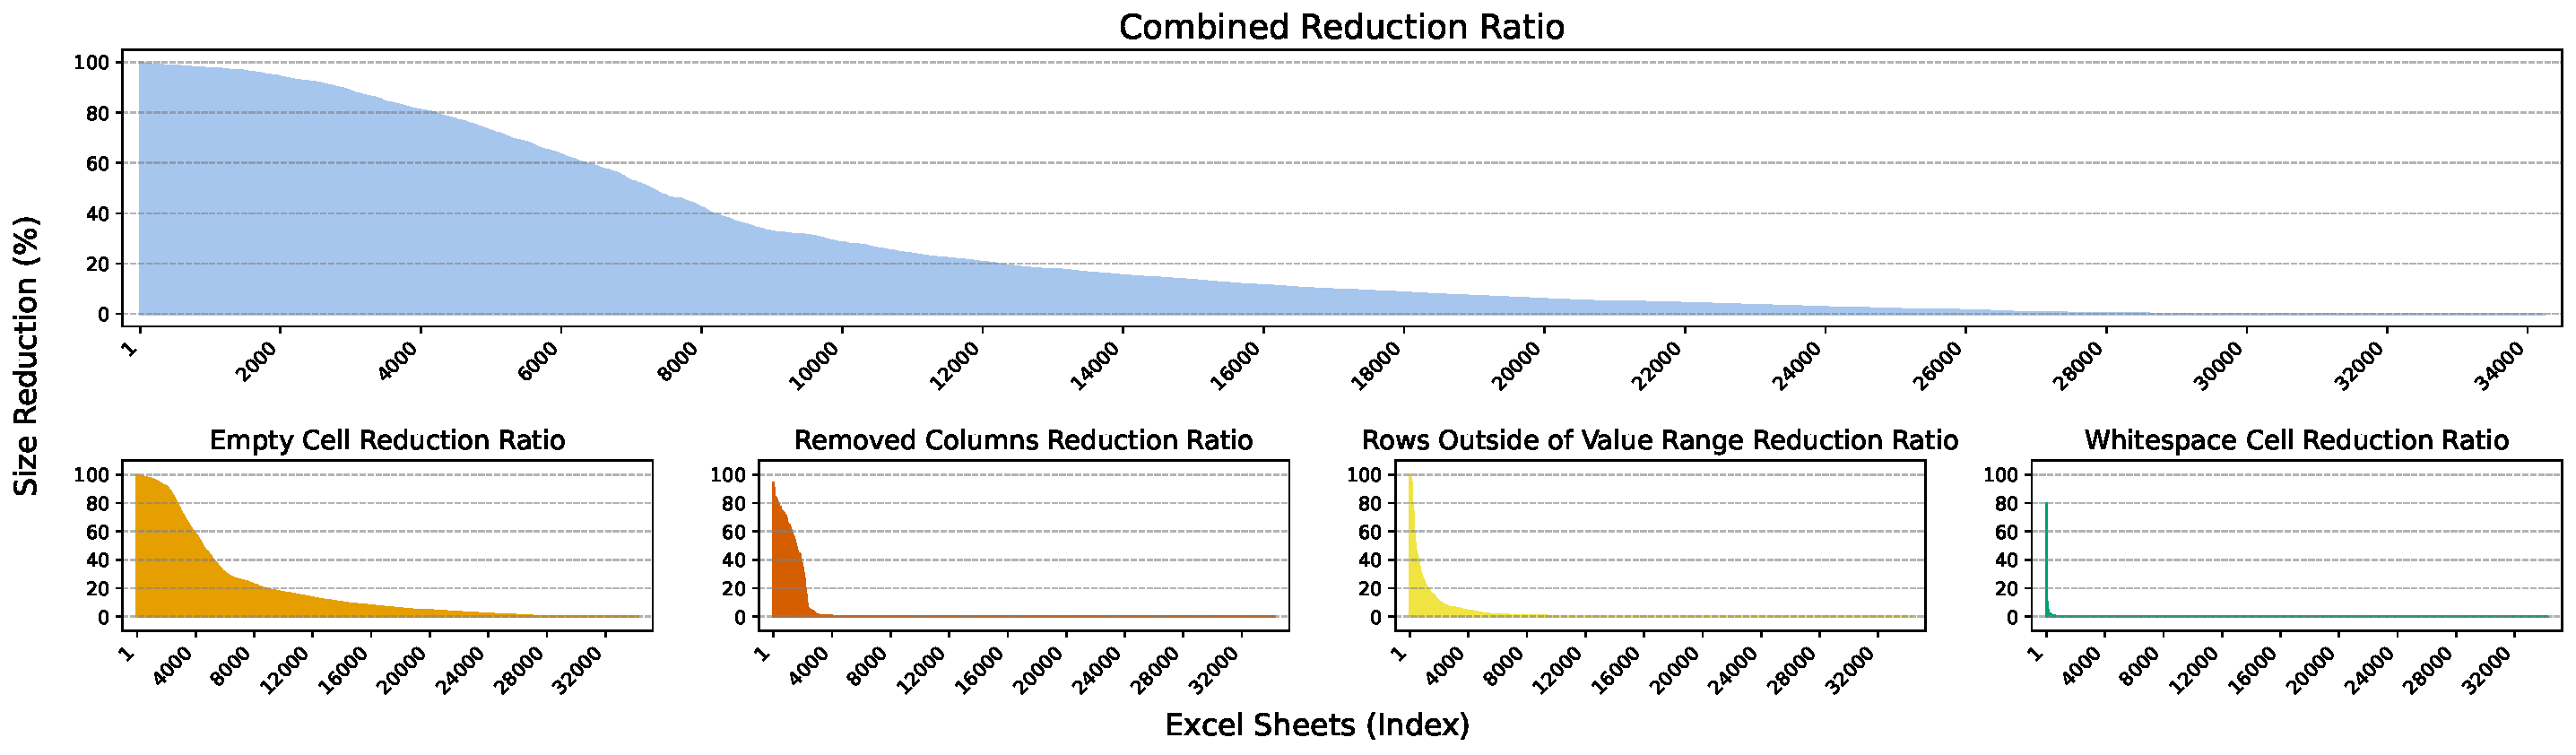
\includegraphics[width=\textwidth]{scripts/analyze_destatis_xlsx_files/charts/combined_chart_distribution_of_size_reduction.pdf}
  \caption{Distribution of Size Reduction Percentages for Excel Sheets}
  \label{fig:size-reduction-chart}
\end{figure*}

\subsection{Multi-process Execution}

Our multi-process execution model relies on a process pool that distributes workbook and per-sheet cleaning tasks across multiple CPU cores. This level of concurrency is only feasible because \texttt{Excel Shrink} operates directly on the raw byte stream using regular expressions, rather than parsing the XML tree structure of each sheet.

If we instead used XML parsing—as in the earlier \emph{Excel Shrink Analyzer} prototype—the memory footprint would already be saturated in single-process mode, with multi-gigabyte workbooks easily exhausting 8–16 GB of RAM on a typical consumer machine. Running 2, 4, or even 12 XML-based cleaning threads concurrently would therefore be impossible. By contrast, our byte-stream approach keeps memory consumption minimal and enables parallel execution even for extremely large workbooks.

Beyond memory efficiency, we further optimised scheduling. When a file with multiple sheets (e.g. 13) is being cleaned, up to 12 sheets can be processed in parallel. As soon as one process finishes its assigned sheet, it immediately fetches the next available task—either another sheet within the same workbook or, if all sheets are already processed, the next workbook in the queue. This dynamic scheduling ensures that no CPU core remains idle, except when the final workbook is being processed.


 














  
\section{Evaluation}
We tested our approach on 1,183 real Excel files from the German Federal Statistical Office (\textit{Destatis})~\cite{original_destatis_xlsx_files},\cite{shrinked_destatis_xlsx_files}, covering year-based directories and containing numerous oversize spreadsheets. Excel Shrink Analyzer Script completed parsing and cleaning those files in 3 hours and 43 minutes while our multithreaded streambased approach using regular expressions took 20 minutes and 42 seconds. This represents a 10x speedup over the single-threaded DOM-Parser driven version. The multithreaded approach also significantly reduced memory usage, as each thread only required a small buffer to process its portion of the file. This improvement allowed us to process larger files that would have exceeded memory limits using the single-threaded approach.



\begin{figure*}
  \centering
  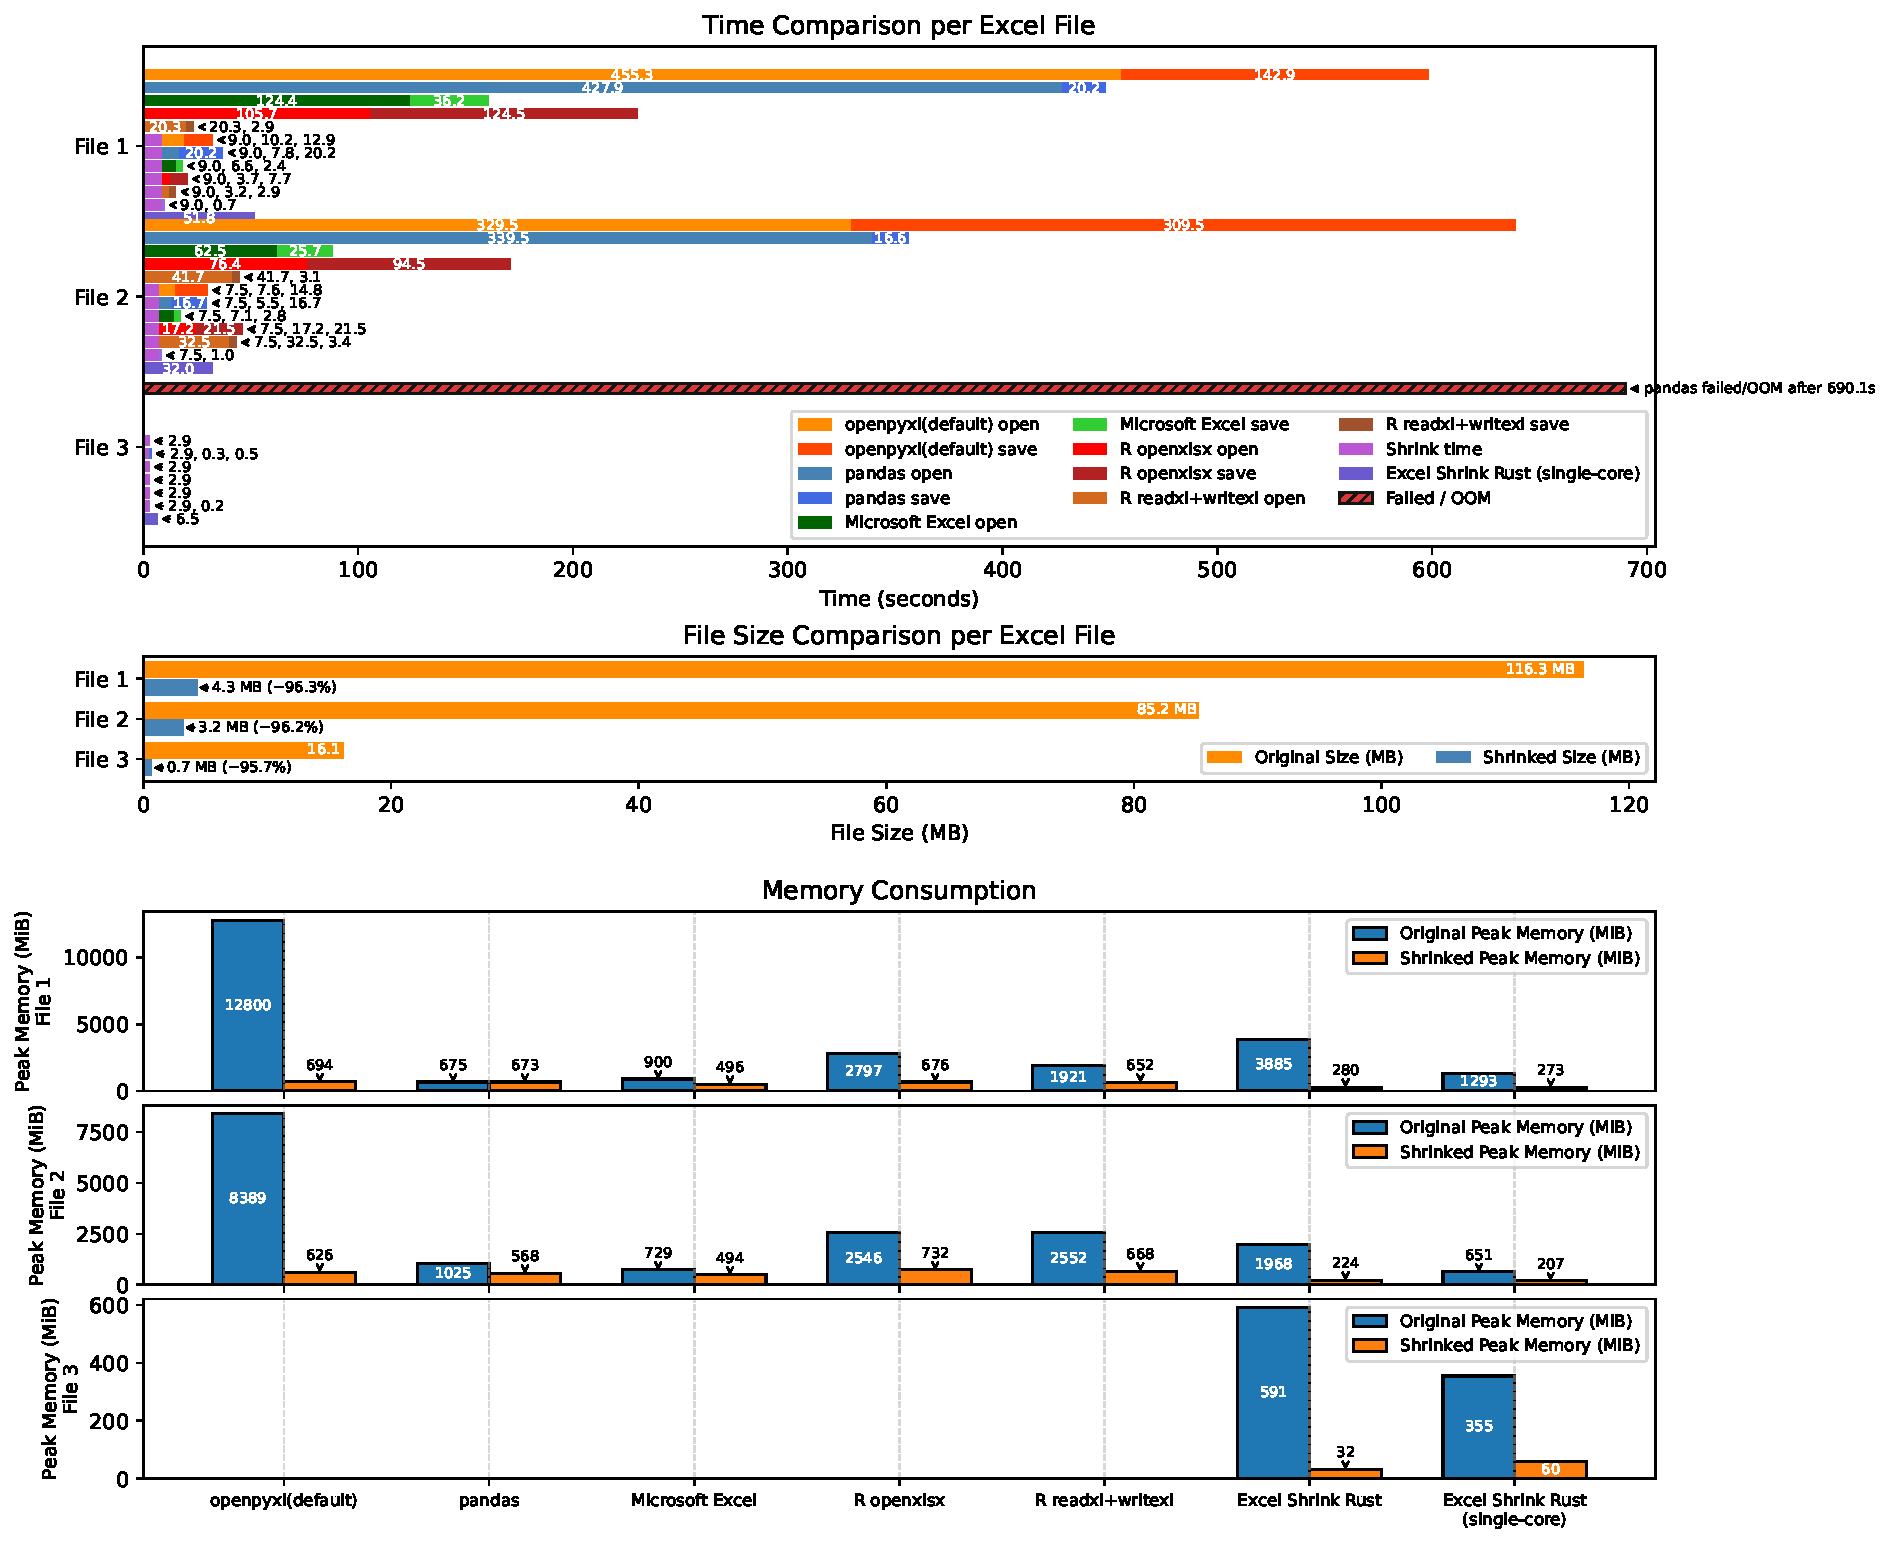
\includegraphics[width=\textwidth]{scripts/loading_times_size_reduction/charts/time_and_filesize_comparison_by_file.pdf}
  \caption{Loading Times and Size Reduction for the 3 Largest \textit{Destatis} Files Before and After applying \textit{Excel Shrink}}
  \label{fig:loading-times}
\end{figure*}


Our primary goal was to quantify the extent of data reduction achieved by \textit{Excel Shrink}, focusing on metrics such as overall size reduction, removal of empty cells, elimination of whitespace cells, deletion of rows outside the value range, and the removal of unnecessary columns. Figure~\ref{fig:size-reduction-chart} presents the distribution of reduction rates (in percentage) for individual worksheets across all these categories. The chart shows that some worksheets experienced reductions approaching 100\% in file size. In particular, one worksheet exceeded a 99.99\% reduction, 16 worksheets surpassed 99.9\%, and 210 worksheets achieved reductions above 99\%. Across all worksheets, the average reduction rate was 25\%. Most of these gains were realized by removing rows that lay outside the range of actual data values.


To further assess the performance improvements enabled by \textit{Excel Shrink}, we identified the two largest files in our \textit{Destatis} dataset \cite{destatis2023Rechnungsergebnisse, destatis2022Verkehrsunfaelle}. Prior to processing, these files measured 85.2~MB and 36.3~MB in their compressed \textit{Excel} (.xlsx) format and expanded to 911~MB and 741~MB when uncompressed. 
Figure~\ref{fig:loading-times} summarises the runtime, size, and memory
consumption for the two representative \textit{Destatis} workbooks before and
after applying \textit{Excel Shrink}.  Each file was processed with six
libraries—\texttt{openpyxl}, \texttt{pandas}, \texttt{Microsoft~Excel},
\texttt{R~openxlsx}, \texttt{R~readxl+writexl}, and our own
\texttt{Excel~Shrink} pipeline—both in their original and cleaned versions.

\paragraph{Loading and Saving Times}
The upper chart shows that \texttt{openpyxl} required by far the longest
execution times, with more than 500 seconds for the largest workbook, whereas
\texttt{pandas} and the R-based libraries performed substantially faster.
After shrinking, the time to open and save the same files decreased for every
library, often by one to two orders of magnitude.
For example, \texttt{R~readxl+writexl} improved from 191.7 s to 7.9 s in the
second file, and \texttt{Excel~Shrink} itself completed a full clean-and-save
cycle in less than 10 seconds.  The second shrink run (“Second~Excel~Shrink
run”) is shown only for completeness and confirms the idempotence of our
cleaning approach—the processing time remains minimal because no further
redundant content is detected.

\paragraph{File Size Reduction}
The middle chart quantifies the reduction in file size. Both workbooks
shrank substantially—from 85.2~MB and 35.4~MB (911~MB and 741~MB uncompressed)
to 2.4~MB and 1.9~MB (20.8~MB and 10.7~MB uncompressed)—corresponding
to 97.2\% and 94.7\% reductions (97.7\% and 98.6\% for the uncompressed sizes).
Such compression not only
reduces storage requirements but also decreases network transfer time
when exchanging files.


\paragraph{Memory Consumption}
The bottom chart shows the peak memory usage for each library before and after shrinking.
Across all tools, the reduction in file complexity led to markedly lower memory requirements.
\texttt{openpyxl} exhibited the highest demand—up to 8.5 GB when opening the uncleaned workbook—posing a serious challenge for consumer-grade computers with 8 GB of RAM.
After shrinking, its peak memory dropped to about 620 MB, making the workbook manageable on typical systems.
For R-based libraries such as \texttt{openxlsx} and \texttt{readxl + writexl}, the original peak consumption of roughly 2.5 GB decreased to below 700 MB.
Even though \texttt{Excel Shrink} is implemented in Python, its memory profile was comparable to that of Microsoft Excel itself for the bloated workbook and became slightly lower than that of Excel for the cleaned workbook.

Overall, these results confirm that \textit{Excel Shrink} not only minimises
file sizes but also enables faster and more memory-efficient processing across
different ecosystems, making large public spreadsheet datasets substantially
more accessible for both analytical and production workloads.






\subsection{Experimental Setup}
\label{sec:experimental-setup}

To evaluate the behavior of \textit{Excel} regarding how the files are interpreted and saved, as well as to test the behavior of the \textit{Add-in} and the new \textit{Check Performance} feature, we tested with two distinct versions of \textit{Excel} from \textit{Microsoft Office}: \textit{Microsoft Office LTSC Professional Plus 2021} and \textit{Microsoft Excel for Microsoft 365 MSO (Version 2409 Build 16.0.18025.20030) 64-bit}. These versions were selected to evaluate compatibility and performance across different Excel environments. Our experiments were conducted on a laptop equipped with an AMD Ryzen 5 Pro 7535U processor (6 cores, 12 threads, 2.9 GHz base clock) and 32 GB of RAM.

\subsection{Comparison with Other Tools for Reducing Bloat}

Excel users lack a straightforward method to identify which cells in a worksheet contain only whitespace characters. To highlight these whitespaces, we have marked cells containing exclusively whitespaces in red within this worksheet, which includes 4,121 such instances (see Figure~\ref{fig:whitespaces})~\cite{destatis2023Konsumausgaben5811109}. Excel Inquire Add-in, Excel Check Performance and NXPowerLite Desktop did not remove Whitespaces, while Excel Shrink identified and removed them.


\begin{figure}[ht]
  \centering
  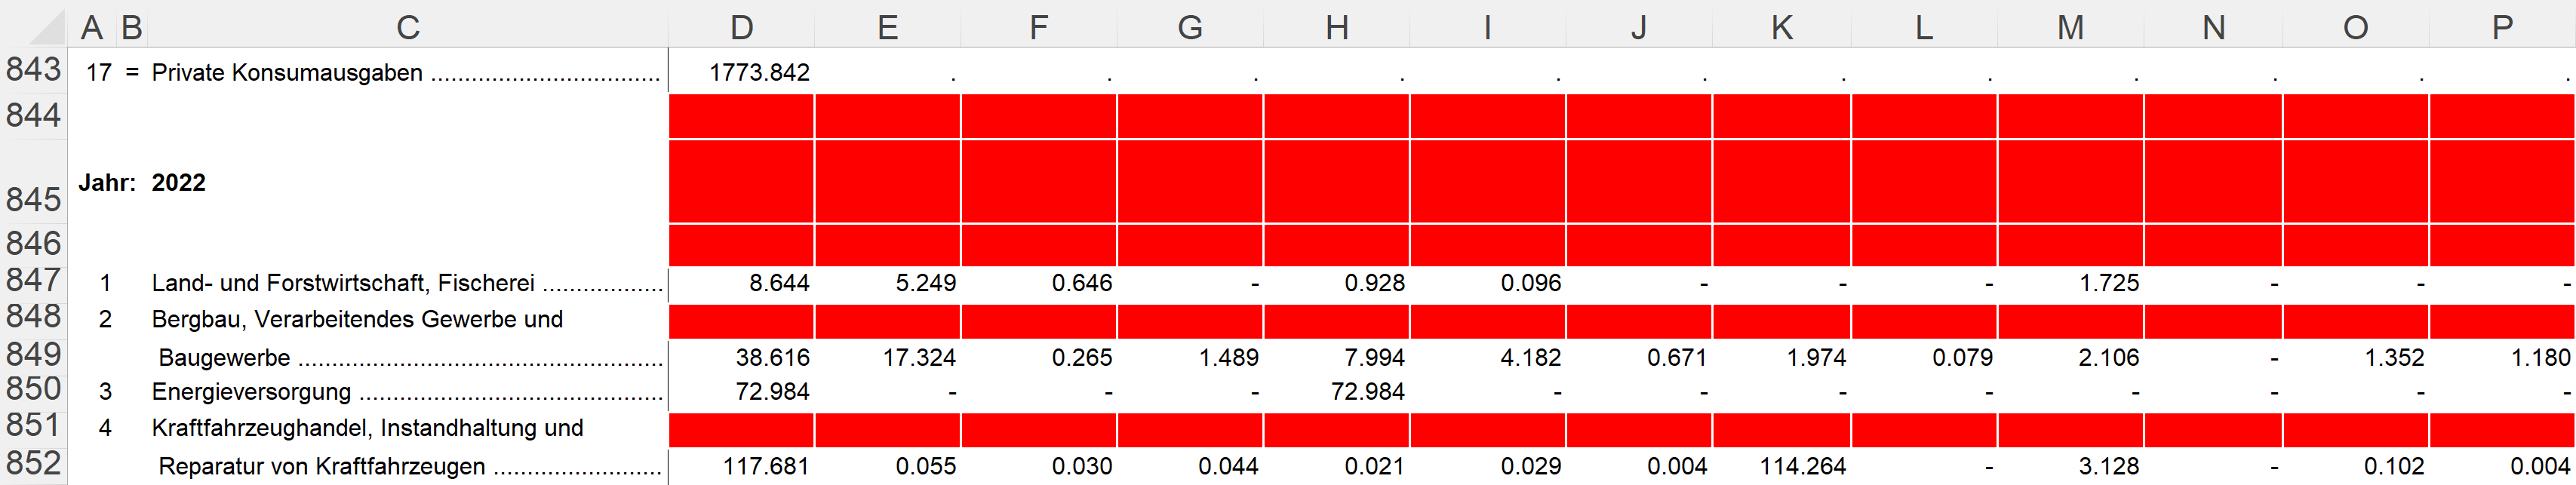
\includegraphics[width=\linewidth]{images/excel_shrink/whitespaces/whitespaces3.png}
  \caption{Cells containing only whitespaces highlighted in red.}
  \label{fig:whitespaces}
\end{figure}%



\subsubsection{Excel Inquire Add-in}

The \textit{Excel Inquire} Add-in, available only in \textit{Office Professional Plus} and \textit{Microsoft 365 Apps for Enterprise}, can remove some redundant content~\cite{o2014excel}.

\textit{Excel Inquire} ignored whitespace cells but can delete empty cell, column, and row definitions. Yet, in certain cases, a significant number of unnecessary elements remain. For example, consider a worksheet serving as a cover sheet, where only the first 77 rows are used and the remaining rows (78 to 65,533(the old limit of row in Excelfiles before it was increased to 1,048,576)) are hidden. Despite being hidden, all these rows and cells are defined in the XML structure, as shown in Listing~\ref{lst:row-65533}.

\begin{lstlisting}[
  language=XML,
  caption={Row 65533 in sheetX.xml},
  label={lst:row-65533},
  basicstyle=\ttfamily\footnotesize,
  frame=none,
  breaklines=true,
  columns=fullflexible,
  showstringspaces=false
]
  <row r="65533" spans="1:7" ht="0" hidden="1" customHeight="1">
    <c r="A65533" s="68" />
    <c r="B65533" s="68" />
    <c r="C65533" s="68" />
    <c r="D65533" s="68" />
    <c r="E65533" s="68" />
    <c r="F65533" s="68" />
    <c r="G65533" s="68" />
  </row>
</sheetData>
\end{lstlisting}

When applying the \textit{Excel Inquire} Add-in to such worksheets, these hidden rows and cells remain. A dialog box reports that because the default row height is \texttt{0}, the tool cannot clean the sheet, causing the operation to be skipped entirely. Excel Shrink successfully removed those cells.

\subsubsection{Excel Check Performance}

The \textit{Check Performance} feature, introduced in \textit{Excel} for the Web and recent desktop versions, can achieve substantial file size reductions~\cite{shirolkar2022check,shirolkar2024make}. However, it often removes cells and rows that influence the spreadsheet’s layout and formatting, thereby altering its visual appearance. This is unacceptable in contexts where maintaining the original look and structure of the spreadsheet is essential.

Figure~\ref{fig:cover_sheet_check_performance} illustrates how \textit{Check Performance} modifies a cover sheet by removing empty rows. Such modifications become problematic when these empty rows serve a functional purpose, such as aligning the layout for printing. In the example shown, the cells responsible for providing space on the cover sheet (Figure~\ref{fig:cover_sheet_check_performance_before}) are removed, as shown in Figure~\ref{fig:cover_sheet_check_performance_after}~\cite{destatis2022Verkehrsunfaelle}. Excel Shrink preserves this layout.

\begin{figure}[ht]
  \centering
  \begin{subfigure}[b]{0.48\linewidth}
    \centering
    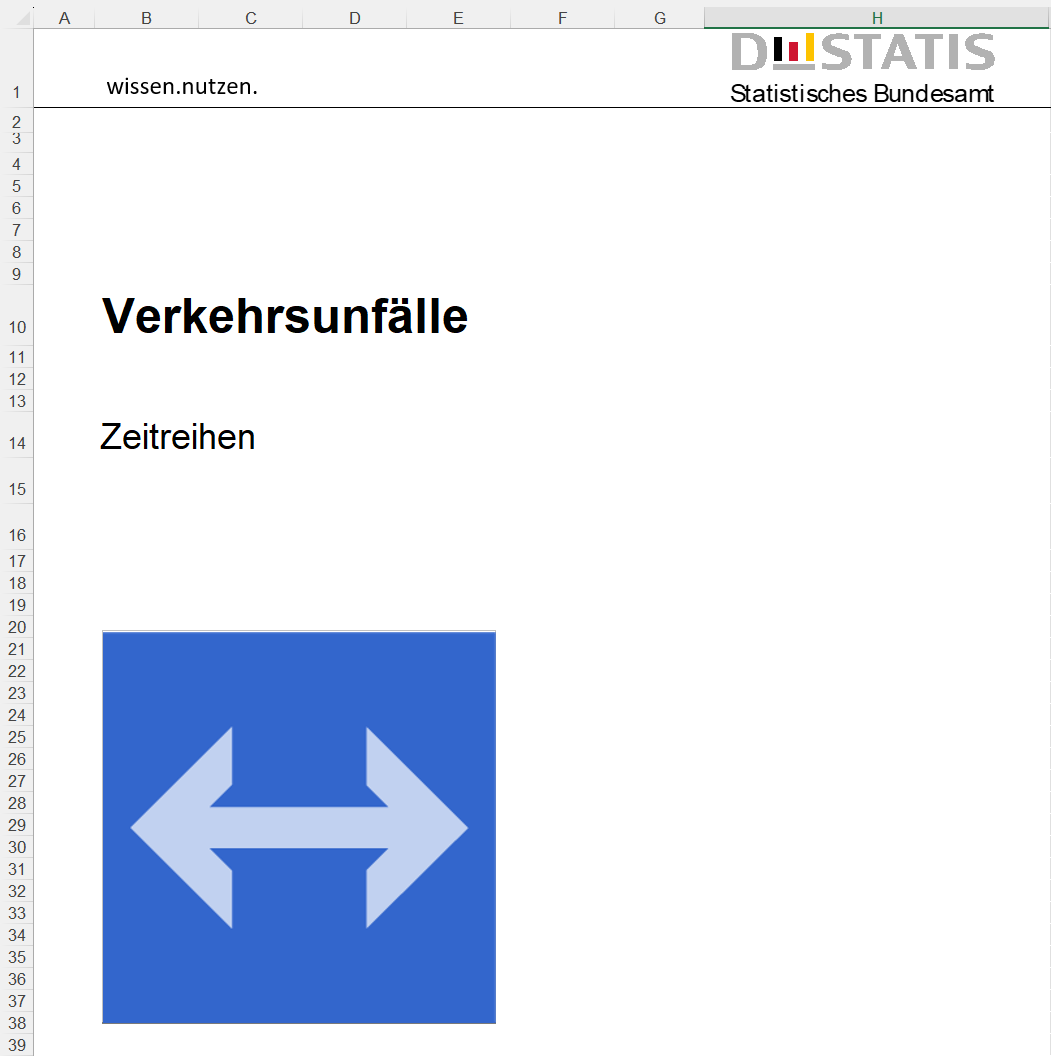
\includegraphics[width=\textwidth]{images/excel_shrink/related_work/performance/verkehrsunfaelle-performance.png}
    \caption{Before Applying Check Performance}
    \label{fig:cover_sheet_check_performance_before}
  \end{subfigure}
  \hspace{0.01\linewidth} 
  \begin{subfigure}[b]{0.48\linewidth}
    \centering
    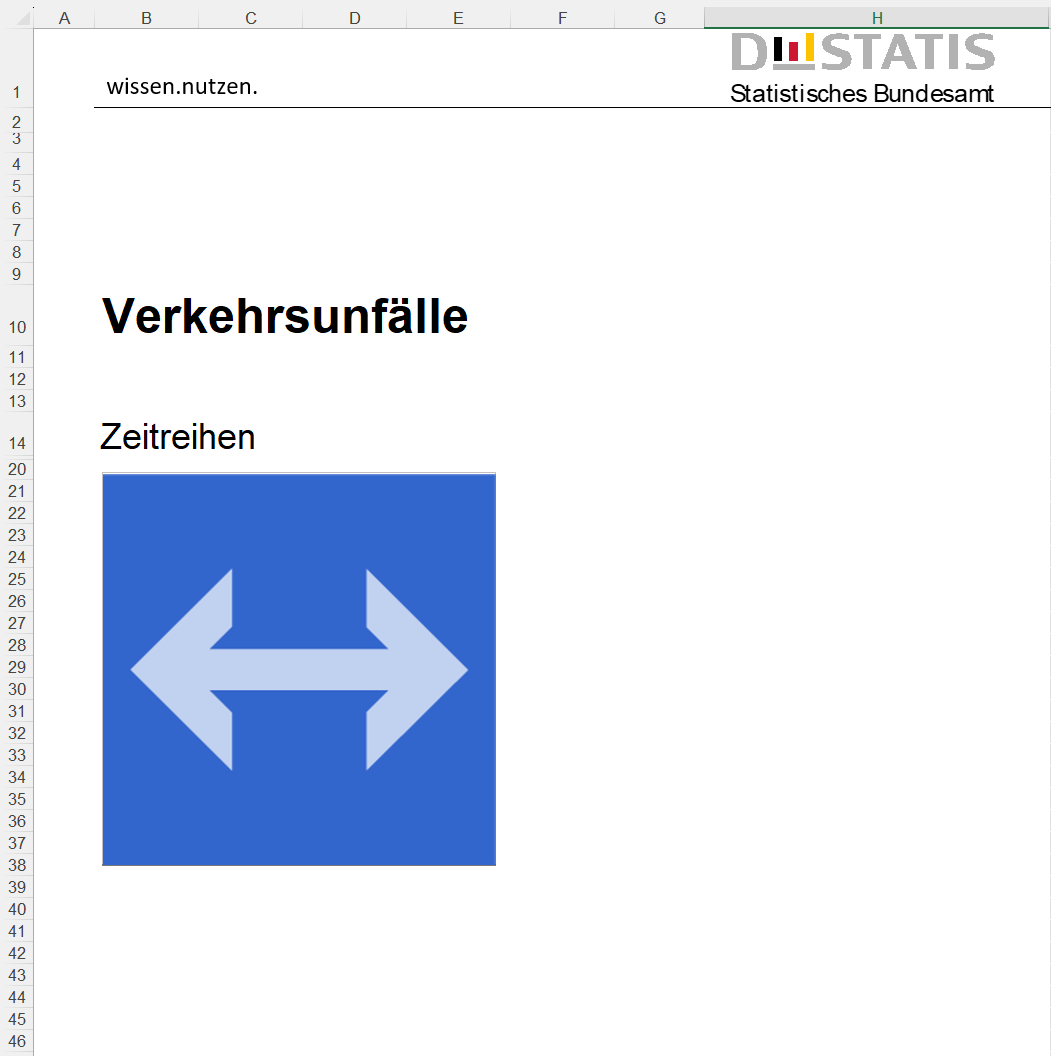
\includegraphics[width=\textwidth]{images/excel_shrink/related_work/performance/verkehrsunfaelle-performance_after.png}
    \caption{After Applying Check Performance}
    \label{fig:cover_sheet_check_performance_after}
  \end{subfigure}
  \caption{Comparison of a Cover Sheet Before and After Applying Check Performance}
  \label{fig:cover_sheet_check_performance}
\end{figure}

As another example, consider a form-like structure composed of several empty cells arranged to form a table, anticipating future data entry~\cite{destatis2023Rechnungsergebnisse}. \textit{Check Performance} removes all borders outside the active data region, resulting in the scenario shown in Figure~\ref{fig:table_no_table}, where the intended table layout is lost. Because Excel Shrink marks all cells as important if they are visible to the user, it does not delete them.

\begin{figure}[ht]
  \centering
  \begin{subfigure}[b]{0.48\linewidth}
    \centering
    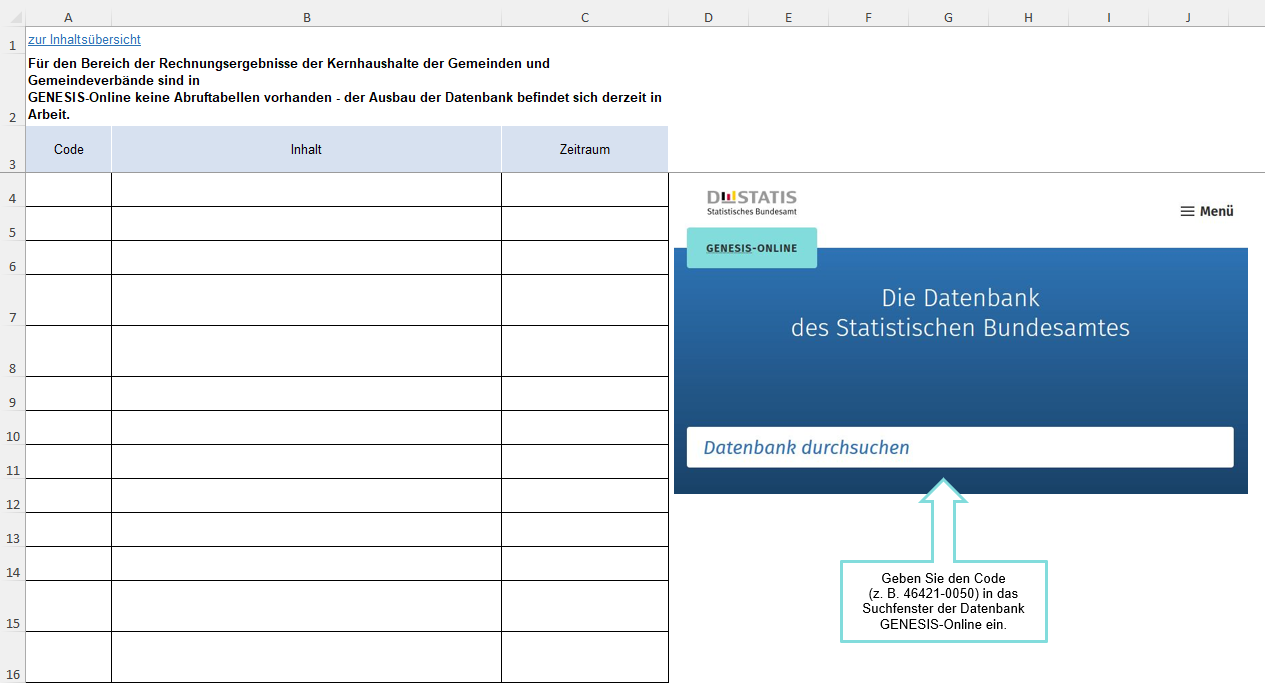
\includegraphics[width=\textwidth]{images/excel_shrink/related_work/performance/table2.png}
    \caption{Before Applying Check Performance}
    \label{fig:table}
  \end{subfigure}
  \hspace{0.01\linewidth} 
  \begin{subfigure}[b]{0.48\linewidth}
    \centering
    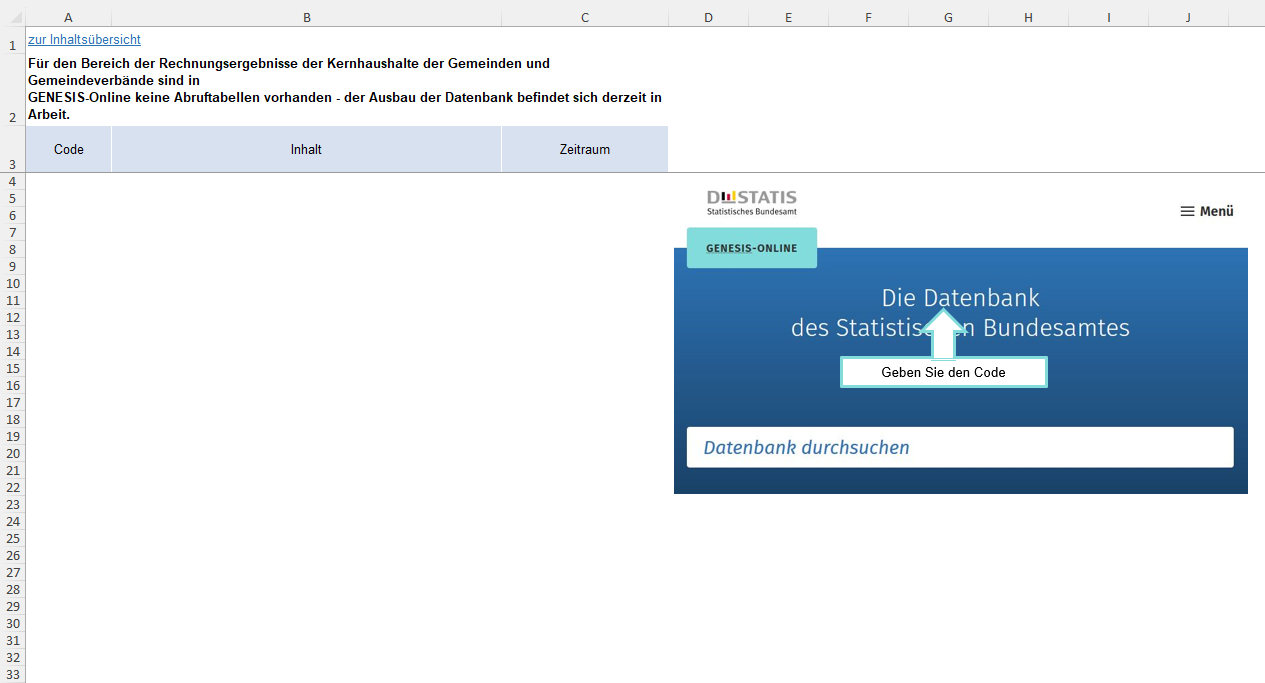
\includegraphics[width=\textwidth]{images/excel_shrink/related_work/performance/no_table2.png}
    \caption{After Applying Check Performance}
    \label{fig:no_table}
  \end{subfigure}
  \caption{Removal of Borders Defining an Empty Table Structure}
  \label{fig:table_no_table}
\end{figure}


\subsubsection{LibreOffice Calc}

Another commonly used tool capable of reading and rewriting Excel workbooks is
\textit{LibreOffice Calc}. When opening and re-saving spreadsheets, Calc internally
parses the XML and reconstructs its own representation of the file, usually resulting in a smaller file size. However, LibreOffice does not fully interpret the
\texttt{applyFill} and \texttt{applyBorder} overwrite flags, which can lead to visualisation errors when a workbook is re-saved.

Figure~\ref{fig:libre_office_apply_fill} shows such a case.
In the original file (Figure~\ref{fig:libre_office_apply_fill_before}),
header cells are shaded in light blue as intended.
After saving the same workbook in LibreOffice Calc
(Figure~\ref{fig:libre_office_apply_fill_after}),
the shading changes to bright green because the
\texttt{applyFill} flag is not respected. Excel Shrink preserves the original appearance.

\begin{figure}[ht]
  \centering
  \begin{subfigure}[b]{0.48\linewidth}
    \centering
    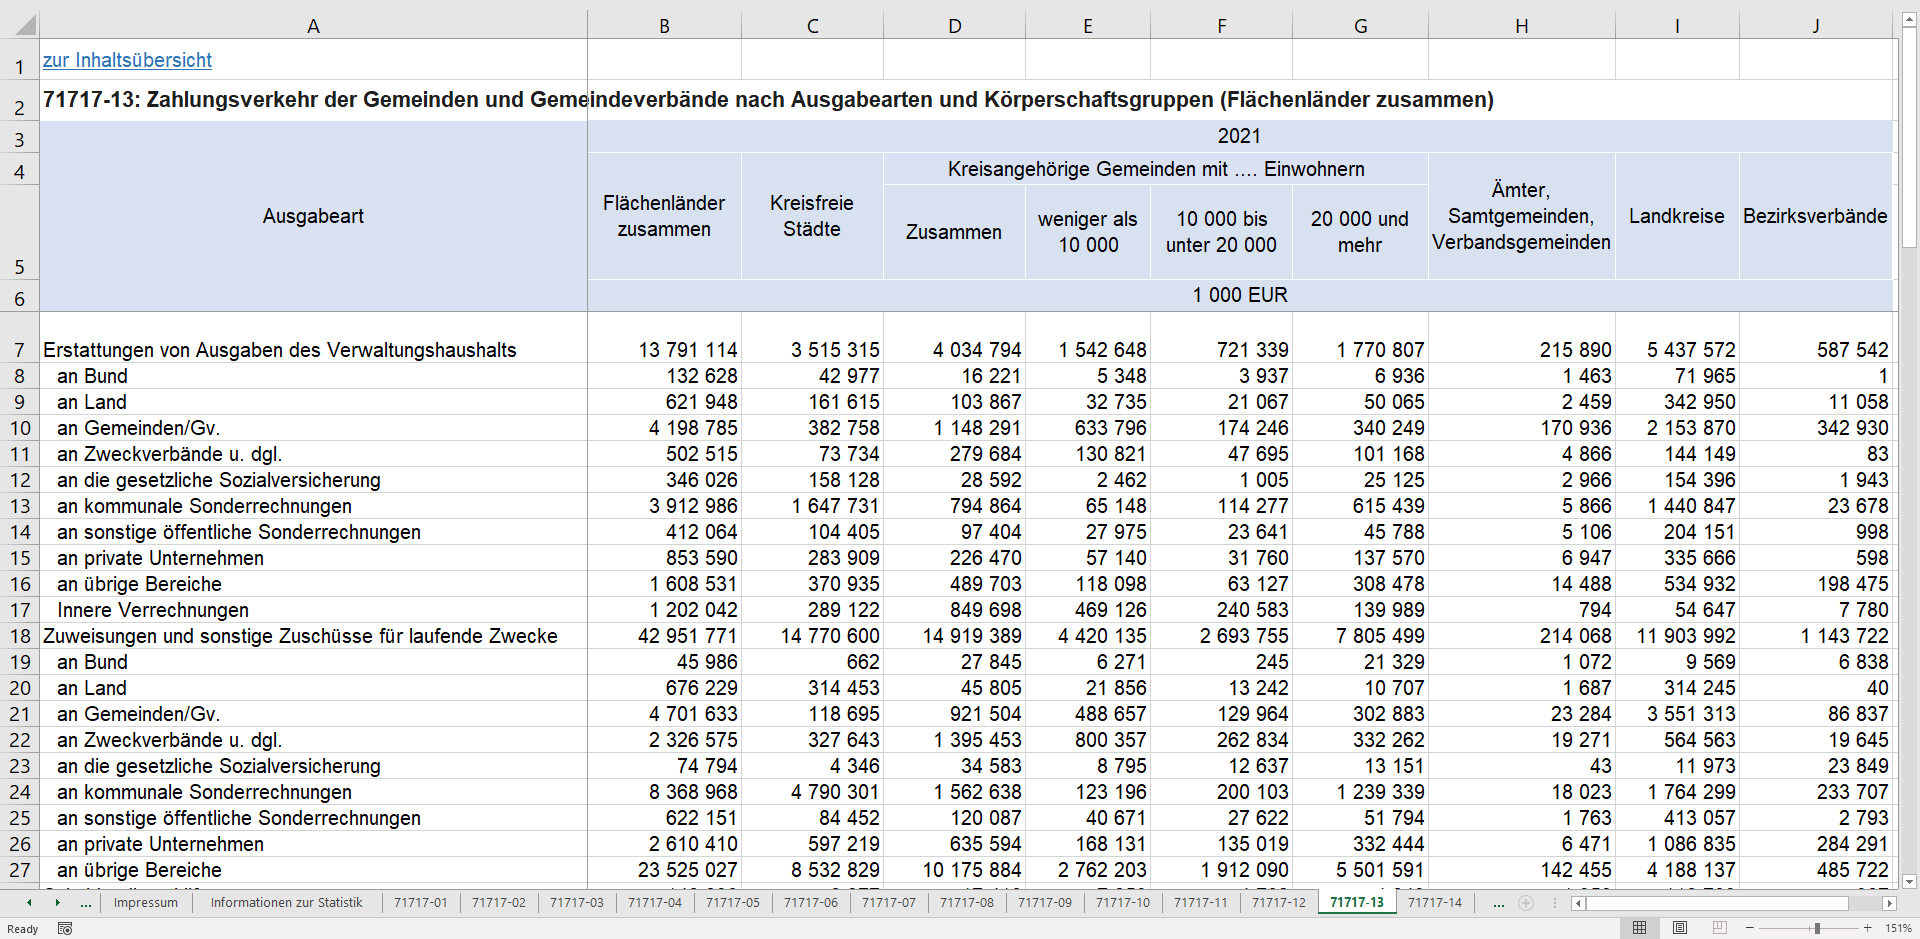
\includegraphics[width=\textwidth]{images/excel_shrink/apply_fill/libre_office_apply_fill_before.png}
    \caption{Before Saving with Libre Office Calc}
    \label{fig:libre_office_apply_fill_before}
  \end{subfigure}
  \hspace{0.01\linewidth} 
  \begin{subfigure}[b]{0.48\linewidth}
    \centering
    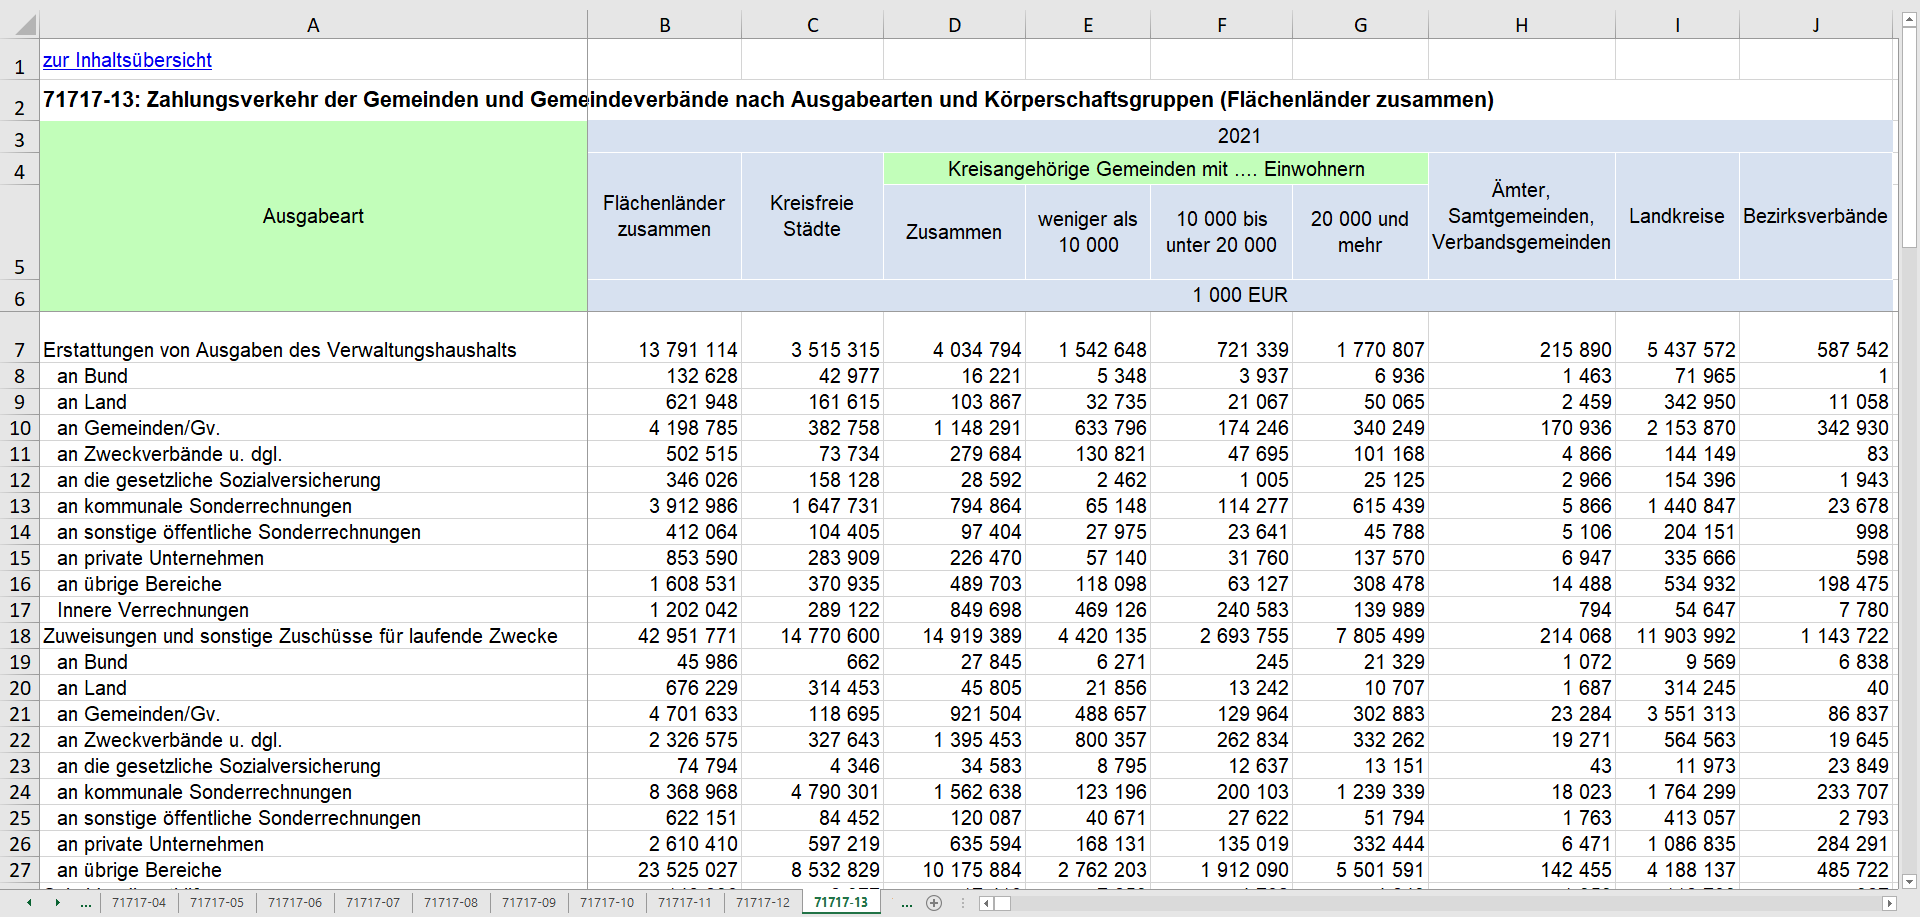
\includegraphics[width=\textwidth]{images/excel_shrink/apply_fill/libre_office_apply_fill_error.png}
    \caption{After Saving with Libre Office Calc}
    \label{fig:libre_office_apply_fill_after}
  \end{subfigure}
  \caption{Visualisation Error Caused by Ignoring \texttt{applyFill} in LibreOffice Calc}
  \label{fig:libre_office_apply_fill}
\end{figure}

\section{Conclusion}
\label{sec:conclusion}

We have presented \textit{Excel Shrink}, a tool that significantly reduces the file sizes of \textit{Excel} sheets by eliminating unnecessary content. Our analysis identified common practices that lead to bloated \textit{Excel} files and demonstrated how targeted removal of redundant data can achieve reductions of up to 99.99\% in real-world Excel files without altering the spreadsheets' appearance while outperforming existing solutions in both file size reduction, preservation of formatting and performance.

\section*{Acknowledgements}

I warmly thank Dr.\,agr.\,Norbert Röder and Dr.\,Johanna Fick for their invaluable guidance and advice on scientific writing, as well as Prof.\,Dr.\,Hardy Pundt and Prof.\,Dr.-Ing.\,Jörg Dörr for their mentorship during this work. I also wish to thank Linus Schmidt for his support in the scientific literature search and for the code experiments we conducted together. Finally, I extend my thanks to the Statistisches Bundesamt (DESTATIS) for enabling the publication of the insights presented here.


\section*{AI-Generated Content Acknowledgement}
We used OpenAI’s ChatGPT 5 solely for language editing and grammar enhancement. No AI-generated content was used in this paper; all scientific ideas, analyses, and conclusions are entirely the authors’ own.



































































































































































































 











\bibliographystyle{IEEEtran}
\bibliography{acmart}


\vspace{12pt}

\end{document}